\documentclass[11pt]{article}
\usepackage[T1]{fontenc}
\usepackage[utf8]{inputenc}
\usepackage{lmodern}
\usepackage[margin=1in]{geometry}
\usepackage{amsmath,amssymb,amsthm,mathtools}
\usepackage{microtype,booktabs,longtable,array}
\usepackage{graphicx,xcolor}
\usepackage{caption}
\captionsetup{font=small,labelfont=bf,textfont=normalfont,labelsep=period,
  justification=justified,singlelinecheck=false}
\usepackage[numbers,sort&compress]{natbib}
\usepackage{xurl}
\usepackage{float,needspace}
\usepackage[hidelinks]{hyperref}
\usepackage{listings}
\setlength{\emergencystretch}{2em}
\definecolor{coderule}{gray}{0.65}
\lstset{basicstyle=\ttfamily\small,columns=fullflexible,keepspaces=true,
  showstringspaces=false,upquote=true,breaklines=true,breakatwhitespace=true,
  frame=tb,rulecolor=\color{coderule},framerule=0.4pt,framesep=6pt,
  xleftmargin=6pt,xrightmargin=6pt,aboveskip=10pt,belowskip=10pt,
  captionpos=b,literate={γ}{{$\gamma$}}1 {≤}{{$\leq$}}1
  {⊢}{{$\vdash$}}1 {₀}{{$_0$}}1}
\newtheorem{proposition}{Proposition}
\newtheorem{example}[proposition]{Example}
\newcommand{\R}{\mathbb R}
\newcommand{\N}{\mathbb N}
\newcommand{\E}{\mathbb E}
\newcommand{\norm}[1]{\lVert#1\rVert}
\newcommand{\src}[1]{\texttt{\nolinkurl{#1}}}
\title{Proof Architecture in the OpenAI Lean Library:\\Representation, Locality, and Semantic Transport}
\author{Robin Gounder\thanks{Correspondence: \href{mailto:robin@gounder.com}{robin@gounder.com}.}\\{\small Vaionex Corporation}}
\date{9 October 2026}
\hypersetup{pdfauthor={Robin Gounder},pdftitle={Proof Architecture in the OpenAI Lean Library: Representation, Locality, and Semantic Transport}}
\begin{document}
\maketitle
\begin{abstract}
What information must a change of representation preserve for a formal
proof to continue? This review studies that question in six developments
from the OpenAI Lean collection: common-base counting, graph switch
chains, the symmetric Mahler inequality, the complete Crouzeix bound,
extended trace cones, and marked character-variety constructions.
We follow the declarations that transport probability laws, computational
bounds, analytic estimates, and coordinate identities to their downstream
uses. The cases expose a division of proof work: mathematical interfaces
establish the hypotheses under which local arithmetic, algebraic, and
finite checks suffice. Elementary examples explain the information these
interfaces must retain. An exploratory survey compares 800 uniformly
sampled OpenAI modules with 8,070 mathematical modules in their pinned
Mathlib dependency. With equal weight per proof-bearing module and joint
standardization by broad subject and proof-length band, arithmetic and
algebra tactics occur in a larger share of extracted named proof bodies
by 22.8 percentage points; the differences are 10.4 points for tactic-mode
proofs and 5.8 for local claims or calculation chains. Comparing these
estimates with subject-only controls separates persistent arithmetic
emphasis from differences associated with proof length. Large numerical
certificate batches also make pooled body frequencies differ sharply
from module averages. Together, source tracing and corpus analysis
identify how established Lean methods are organized in this collection
and give readers a practical way to inspect the mathematical obligations
behind a formal theorem.
\end{abstract}

\noindent\textbf{Keywords:} formalized mathematics; Lean; proof architecture; proof automation; semantic preservation; mathematical interfaces.
\section{Introduction}

A formal proof often changes the language in which its objects are
represented. A graph becomes a Boolean matrix; an algebraic wedge product
becomes a continuous bilinear operator; a randomized estimator becomes a
program reading addressed tape bits. The next argument needs more than a
new description of the object. It needs a theorem preserving the
particular quantity or operation on which that argument depends.

We call such correspondences preservation interfaces. An interface
specifies the relation between two representations and exposes the
information available to a later construction. To transfer an accuracy
guarantee, it must preserve the relevant event probability; equality of
output laws supplies a reusable sufficient condition. To differentiate a
field, it must provide appropriate local agreement. To transport an
equation in named coordinates, it must identify the coordinate maps.
These requirements explain both the mathematical content and the formal
shape of the interfaces studied here.

Six developments in the OpenAI Lean collection provide the comparison
\citep{OAIRepository}. Common-base counting and graph switch chains
connect finite representations to probabilistic guarantees. The Mahler
and Crouzeix arguments connect algebraic identities to differentiation,
integration, and norm estimates. Trace ideals and marked character-variety
diagrams reconstruct or transport algebraic data. The first four selected
statements are public theorem endpoints; the last two are support results.
Keeping these roles explicit allows the comparison to follow the
mathematical work performed by each selected construction.

Three questions guide each case: what does the intermediate representation
retain, which theorem relates it to the intended object, and how is that
theorem used in the next step? The case studies answer these questions
through source declarations and worked mathematical examples. A separate
exploratory survey compares the written proof methods of 800 uniformly
sampled OpenAI modules with the pinned Mathlib dependency. It distinguishes
average within-module practice from body frequencies dominated by large
certificate batches, then examines broad subject and proof-length
composition. The two analyses serve mathematicians reading formal source
and formalizers designing reusable interfaces.

Together, they describe a division of proof work. Representation and
preservation lemmas make the hypotheses of a local calculation available;
simplification, arithmetic tactics, or exact decision procedures then
check the resulting obligation. Arithmetic and algebra tactics remain
substantially more prevalent after joint subject and length controls.
The corresponding differences in tactic blocks and intermediate claims
are smaller under these controls. Source examples explain how such
devices operate within particular proofs: the construction determines
which goals reach a tactic and why the available hypotheses suffice.

Companion reviews assess the proposed mathematical advances against
prior results \citep{GounderFrontiers2026} and examine counting and
sampling applications \citep{GounderCounting2026}. The present review
uses common bases, Mahler, and Crouzeix to study a different question:
how the formal source connects its mathematical representations and
organizes the proof obligations between them.

The comparison builds on established accounts of formalization. Lean
combines dependent type theory with an extensible elaborator and a
programming language \citep{deMouraUllrich2021}; Mathlib supplies a shared
mathematical vocabulary \citep{mathlib2020}.
\citet{AvigadEtAl2024Anatomy} trace a linear-algebra example through
formal proof, generalization, and connection to an existing Mathlib
theorem. \citet{CommelinTopaz2024} explain how usable specifications
support mathematical construction and collaboration. Here we compare
the mathematical payload of preservation statements across several
settings and relate their local uses to a corpus-level method profile.

The odd-order theorem and Kepler conjecture establish precedents for
large proof decompositions and verified computation
\citep{GonthierEtAl2013,HalesEtAl2017}. Lean formalizations of perfectoid
spaces and schemes illustrate the importance of representation choices
\citep{Perfectoid2020,Schemes2021}. These precedents frame the novelty
question in this review: which established device is used, what
project-specific information does its interface preserve, and what later
step becomes possible because that information is available?

Section~\ref{sec:method} describes selection and evidence.
Section~\ref{sec:cases} begins with the overview in
Table~\ref{tab:overview}, then develops the six cases.
Section~\ref{sec:profile} compares source-written proof methods with
Mathlib, including joint composition controls and certificate
concentration. Section~\ref{sec:worked} isolates the cases' preservation
requirements in elementary examples. Section~\ref{sec:discussion}
connects the mathematical and empirical findings and develops guidance
for new formalizations.

\section{Sources, selection, and reading method}
\label{sec:method}

Each case follows a chain consisting of an initial representation, a
preservation statement, and its downstream use. Selection was purposive:
a candidate had to expose all three parts and a mathematically meaningful
change of representation. We sought contrasting preservation requirements
across mathematical settings so that the comparison would explain why
different interfaces need different hypotheses.

We read backwards from each selected conclusion to its definitions and
hypotheses, then forwards through the constructions supplying those
hypotheses. This separates the established mathematical device, the
specific relation proved in the development, and its use in a later
argument. Evidence ledgers retain declaration names, source excerpts,
line ranges, and Git blob identifiers. Matching downloaded files to these
identifiers makes the source locations reproducible.

Discovery proceeded from endpoint inspection to deeper tracing of
candidate interfaces. The irrationality-exponent-of-$\pi$ and
two-point-correlation endpoints were considered but excluded because
their mechanisms had not been traced to comparable depth. The six-case
selection therefore supports a focused comparison of interfaces.
Section~\ref{sec:profile} addresses prevalence separately through a
uniform path sample, with explicit extraction units and feature
definitions. This division keeps purposive mathematical analysis distinct
from estimates about the wider source population.

The key reading task is to distinguish an interface from its
instantiation. When an analytic lemma takes a flux identity or resolvent
estimate as input, the analysis follows the endpoint's construction of
that input. Likewise, a witness selected by classical choice is traced
to its existence theorem. This identifies which hypotheses remain in
the final statement and which are supplied within the proof.

All six cases are studied through declaration and dependency analysis.
Their transitive \src{OAI} import closures are retained, and the evidence
ledgers identify the bodies inspected. The worked examples in
Section~\ref{sec:worked} include arithmetic and finite-law lemmas checked
with Lean 4.34.1. A separate experiment compiles three unchanged upstream
trace-cone modules and an importing corollary using the pinned Mathlib
revision. The data and code availability statement records the source
provenance and the scope of these complementary checks.

Blueprints link informal arguments to formal declarations and
dependencies \citep{MassotLeanBlueprint}; LeanArchitect studies
automation of that connection \citep{ZhuEtAl2026}. Our ledgers serve as
source locators for the selected interfaces. The review adds the
mathematical explanation: the equations, normalizations, and hypotheses
that make each transition useful to the next argument.

\Needspace{35\baselineskip}
\section{Six mathematical interfaces}
\label{sec:cases}

Table~\ref{tab:overview} summarizes the cases in three pairs: probability
and computation, analysis, and reconstruction of algebraic data.
Each account follows the objects through a preservation statement to
its mathematical use. The graph-table calculation and Crouzeix energy
cancellation are developed within their cases; Section~\ref{sec:worked}
returns to the other interfaces through smaller examples.

\begingroup
\setlength{\intextsep}{22pt}
\setlength{\abovecaptionskip}{10pt}
\setlength{\belowcaptionskip}{12pt}
\begin{table}[H]
\small
\centering
\renewcommand{\arraystretch}{1.14}
\caption{Overview of the selected formal statements and the information
preserved by each bridge.}\label{tab:overview}
\begin{tabular}{@{}p{0.18\textwidth}p{0.38\textwidth}p{0.37\textwidth}@{}}
\toprule
Development & Representation bridge & Mathematical work exposed\\
\midrule
Common bases\newline Endpoint & Matroid transversals; finite random trees;
oracle expressions; physical random tapes. & Output-law preservation joins
bit-cost bounds and a fixed-program specification.\\[7pt]
\midrule[0.3pt]\addlinespace[7pt]
Graph switches\newline Endpoint & Fixed-degree graph cells;
$2\times2$ Boolean matrices; conditional averaging operators. & A finite
count isolates one exceptional direction per fiber; compensated estimates
control its global contribution.\\[7pt]
\midrule[0.3pt]\addlinespace[7pt]
Mahler\newline Endpoint & Ordered shuffle forms; continuously bundled
fields; boundary-local extensions. & Exact slot identifications preserve
derivatives, signs, and multiplicities; locality makes Stokes applicable.\\[7pt]
\midrule[0.3pt]\addlinespace[7pt]
Crouzeix\newline Endpoint & Amplified polynomial evaluation;
rectangular compressions; Fourier coefficient energies. & Finite dual
witnesses and positive blocks give a scalar cancellation; outer domains
remove strict-containment assumptions.\\[7pt]
\midrule[0.3pt]\addlinespace[7pt]
Trace ideals\newline Support result & Closed ideals; idempotent
extended traces; positive cuts and scalar limits. & Algebraic recovery of
ideals combines with canonical convergence to identify transported ideals.\\[7pt]
\midrule[0.3pt]\addlinespace[7pt]
All seams\newline Support result & A shared splitting witness;
named graded maps; rebased matrices and produced diagram values. & Eight
local seam families cover the constructed diagram; equality transport
retains its named maps.\\
\bottomrule
\end{tabular}
\end{table}
\endgroup

\subsection{Common bases: from a matroid representation to physical random tapes}
\label{sec:common-bases}

The common-bases development follows an approximate count all the way to a
fixed oracle program, its bit costs, and the tape positions supplying its
randomness \citep{OAICommonBases}. Three descriptions of the computation
are kept explicit: the mathematical estimator, a finite random experiment,
and the compiled machine. Successive interfaces track the counted objects,
the output law, and execution on a given input through this pipeline.

\paragraph{Encoding the counting problem.}
The mathematical problem is to count the common bases of two equal-rank matroids $M_1,M_2$ on an enumerated ground set $E=\operatorname{Fin}n$. The first representation replaces two simultaneous base conditions by one base condition. On $E\sqcup E$, set
\[
 N=M_1\oplus M_2^*,\qquad
 T(A)=\operatorname{inl}(A)\cup\operatorname{inr}(E\setminus A).
\]
The source proves that $T(A)$ is a base of $N$ exactly when $A$ is a base of both input matroids.\footnote{\href{https://github.com/openai/math/blob/fd4aeeb2ee4fc729c18d98444fed42fd0529eeeb/lean/OAI/Combinatorics/MatroidCounting/CommonBases.lean\#L7156-L7167}{Base correspondence and the rank of the paired matroid}.} Equal ranks give $r(N)=n$, while every transversal $T(A)$ has size $n$. Consequently the deficiency $d(A)=n-r_N(T(A))$ vanishes precisely at the objects being counted. Explicit equivalences between subsets, finite subsets, and transversals transfer both cardinalities and partition sums. If $Z$ is the common-base count, the resulting annealing partition function satisfies
\[
 Z\leq \sum_{A\subseteq E}q^{d(A)}\leq Z+2^nq,
 \qquad 0\leq q\leq1.
\]
The partition function now has a direct relation to the desired count:
zero-deficiency terms contribute exactly $Z$, and every other term is at
most $q$. The doubled ground set also supplies the exchange space. A plain
state selects one element from each pair; a defect state has one empty
pair, one full pair, and singleton choices elsewhere. The walk passes
through paired defects before a hitting construction returns it to plain
states. This separates the space convenient for local moves from the
transversals whose weighted count is estimated.

A greedy routine next computes rank from independence queries. Its
correctness theorem identifies the implemented deficiency and annealing
weights with the mathematical ones. A sampled zero-deficiency witness
serves as the estimator's final guard. Because such a witness is a common
base, this guard enforces the zero-count conclusion on every execution,
including tapes outside the high-probability accuracy event.

\paragraph{From experiments to a bounded program.}
Finite random experiments are trees with uniform choices at their internal
nodes. The bounded implementation gives each draw a bank of rejection
trials. Its fit condition bounds the number of successive draws by $M$
and requires $H\geq\lceil\log_2 a\rceil$ trial bits for each positive draw
arity $a$. With $D$ trials per draw, the observable loss is at most
$M2^{-D}$ for values in $[0,1]$. The width condition ensures that a trial
can represent every outcome; increasing the number of undersized trials
would not repair that defect. A separate reindexing relation permits
permutations of outcome labels and proves expectation preservation.
Consequently, the walk and its implementation may enumerate choices
differently while agreeing in law.

In the expression language, randomness becomes explicit input. Evaluation
takes a value and a random bank and returns an optional result together
with the unused bank. A realization theorem relates this deterministic
execution, bank by bank, to the random tree. For a Metropolis step, the
proof follows the proposal, acceptance calculation, Bernoulli choice, and
lazy branch. Composition with the witness guard then gives the complete
estimator. Law preservation and bankwise execution preservation enter at
different layers of the same construction.

Compilation preserves the encoded output and supplies a cost bound.
The constructed nine-register stack machine implements the expression
language by structural simulation, including its list folds. Source
evaluation returns both a value and a charge; the machine produces that
value within the recorded charge. This makes resource use part of the
simulation statement, ready for the polynomial-bound argument.\footnote{\href{https://github.com/openai/math/blob/fd4aeeb2ee4fc729c18d98444fed42fd0529eeeb/lean/OAI/Combinatorics/MatroidCounting/CommonBases.lean\#L16459-L16620}{Cost-bearing compiler correctness}.}

\paragraph{From semantic preservation to a polynomial cost bound.}
Bounding the charge requires control of intermediate representations. The recursive
predicate $\operatorname{Safe}(O,S,e,x)$, with oracle $O$, width bound
$S$, expression $e$, and input $x$, bounds the encoded widths of the input and
every successful output, and requires safety of the subevaluations actually
used. For a composition it bounds the intermediate result; for a fold it
requires the invariant after each accumulator update. If the body charge
is at most $E$ and these widths are at most $S$, the fold lemma gives
\[
  c_{\mathrm{fold}}\leq |\mathrm{xs}|\,(7+12S+E).
\]
The encoding bounds list length by width, so this estimate can be composed
through structural induction on the fixed expression. The width
certificate turns the cost-bearing simulation into a polynomial charge
bound.\footnote{See
\href{https://github.com/openai/math/blob/fd4aeeb2ee4fc729c18d98444fed42fd0529eeeb/lean/OAI/Combinatorics/MatroidCounting/CommonBases.lean\#L16855-L16904}{\src{Safe} and the fold-charge proof}, and
\href{https://github.com/openai/math/blob/fd4aeeb2ee4fc729c18d98444fed42fd0529eeeb/lean/OAI/Combinatorics/MatroidCounting/CommonBases.lean\#L17079-L17092}{the structural polynomial bound}.}

The source packages these certificates as \src{PolySafe}: a polynomial
$p$ takes an input parameter $S$ to an admissible width $p(S)$.
Polynomial substitution supports composition. A further interface,
\src{AttrSafe}, carries numerical predicates alongside the width bound.
This matters for value-indexed operations: an exponent can be very large
despite a short binary encoding. The exponentiation lemma consequently
assumes that the exponent itself is at most $S$. The estimator's attribute
bounds three parameter fields, and its proof transports those bounds
through exponentiation, range construction, and ratio products.
In \src{attrSafe_compose}, the next width parameter is enlarged to
$g(S)=p(S)+S$; monotonicity of the numerical attribute carries its
information to that larger parameter. Thus a usable complexity interface
preserves both encoded size and the value constraints needed by the next
operation.\footnote{See
\href{https://github.com/openai/math/blob/fd4aeeb2ee4fc729c18d98444fed42fd0529eeeb/lean/OAI/Combinatorics/MatroidCounting/CommonBases.lean\#L17689-L17706}{\src{PolySafe}},
\href{https://github.com/openai/math/blob/fd4aeeb2ee4fc729c18d98444fed42fd0529eeeb/lean/OAI/Combinatorics/MatroidCounting/CommonBases.lean\#L22444-L22466}{attribute composition}, and
\href{https://github.com/openai/math/blob/fd4aeeb2ee4fc729c18d98444fed42fd0529eeeb/lean/OAI/Combinatorics/MatroidCounting/CommonBases.lean\#L24280-L24308}{the exponent and estimator attributes}.}

\paragraph{From output laws to successful tapes.}
The final probabilistic interface connects the program to its accuracy guarantee. Let $V$ be the canonical bounded experiment, and let $v$ be the rational output function implemented by the postamble. The certificate asserts
\[
 \E_w\,\varphi(v(w))=\E_b\,\varphi(V(b))
 \quad\text{for every }\varphi:\mathbb Q\to\R,
\]
where both expectations are finite uniform averages. It also records source execution and nonnegativity, including zero output when $Z=0$.\footnote{\href{https://github.com/openai/math/blob/fd4aeeb2ee4fc729c18d98444fed42fd0529eeeb/lean/OAI/Combinatorics/MatroidCounting/CommonBases.lean\#L25962-L25968}{The output certificate}.} The universal observable interface transports the output distribution through changes of enumeration and bank layout.

The machine correspondence reaches actual tape addresses. For $m$ total gathered bank bits, there is a start offset $s$, fixed before quantifying over tapes, such that every tape $\beta:\N\to\{0,1\}$ produces
\[
 v\bigl(\operatorname{physicalWord}(s,m,\beta)\bigr),\qquad
 \operatorname{physicalWord}(s,m,\beta)(i)
   =\beta\bigl(s+3(m-1-i)+1\bigr),\quad i<m.
\]
The reversal comes from pushing bits onto a stack; the stride three reflects the sampling loop's instructions. The proof supplies $s+3m+1\leq B$. Injectivity of these positions shows that a uniform length-$B$ tape induces a uniform length-$m$ word.\footnote{\href{https://github.com/openai/math/blob/fd4aeeb2ee4fc729c18d98444fed42fd0529eeeb/lean/OAI/Combinatorics/MatroidCounting/CommonBases.lean\#L25658-L25687}{Physical tape positions and their uniform law}; \href{https://github.com/openai/math/blob/fd4aeeb2ee4fc729c18d98444fed42fd0529eeeb/lean/OAI/Combinatorics/MatroidCounting/CommonBases.lean\#L26027-L26069}{the machine correspondence}.} Here $m$ counts bank bits, whereas $B$ bounds complete machine execution.

The endpoint quantifies over one fixed program and constants $C,a$ before
the input matroids, oracle, and rational parameters
$0<\varepsilon,\delta<1$. For an exact independence oracle and matroids
with full ground set and supplied common rank $r$, the resource bound is
\[
 B=C\bigl(1+n+\ell+\lceil\varepsilon^{-1}\rceil
       +\operatorname{clog}_2\lceil\delta^{-1}\rceil\bigr)^a,
\]
where $\ell$ is the encoded input length and $\operatorname{clog}_2$ is
the ceiling binary logarithm. Execution on every infinite tape produces
an output within $B$, with at most $B$ oracle calls and bit operations.
For a length-$B$ word, let $\operatorname{out}(w)$ denote this output on
the word's zero extension. Substituting the accuracy indicator in the
observable identity yields
\[
 \#\{w\in\{0,1\}^B:(1-\varepsilon)Z\leq\operatorname{out}(w)
                  \leq(1+\varepsilon)Z\}
 \geq(1-\delta)2^B.
\]
The specification packages this success count with the universal resource and zero-output guarantees.\footnote{\href{https://github.com/openai/math/blob/fd4aeeb2ee4fc729c18d98444fed42fd0529eeeb/lean/OAI/Combinatorics/MatroidCounting/CommonBases.lean\#L110-L132}{The fixed-program and finite-tape specification}.} Verified compilation and probabilistic semantic preservation are established methods \citep{Leroy2009,CakeML2014,CertiCrypt2009,EasyCrypt2011}. Expectation-functional semantics for randomized programs is also established
\citep{AudebaudPaulinMohring2009}. In Lean, SampCert separates sampling
procedures from normalized distribution semantics and proves exact sampler
laws \citep{deMedeirosEtAl2025}. Its \src{SLang} represents a program by an
unnormalized mass function; normalization and equalities between sampler
laws support downstream privacy reasoning. The common-base development
instead carries its bounded random experiment through a costed expression
language to a fixed stack machine. A close compiler precedent is Zar,
which translates probabilistic programs through choice-fix trees and
interaction trees to random-bit samplers, proving equidistribution in
Coq \citep{BagnallStewartBanerjee2023}. Here the comparison turns on the
specification carried through the pipeline: intermediate widths and
numerical attributes, an every-tape resource bound, and the finite count
of accurate tapes. The distinctive evidence is the
concrete integration: the proof carries the counting quantity through oracle code, width bounds, and physical tape coordinates to an exact finite success count. Sections~\ref{sec:tape-example}--\ref{sec:success-budget} isolate the uniformity, law, and error-budget arguments behind this last step.

\subsection{Graph switches: a local table and a fiberwise error direction}
\label{sec:switch-chain}

The graph case studies how two conditional averages interact. Its
switch-chain development connects a four-vertex representation to a
spectral estimate \citep{OAISwitch}. The chain stays put with probability
$1/2$; otherwise it chooses uniformly a four-vertex set and an ordered
pair of distinct perfect matchings on it. It replaces the first matching
by the second when the removed edges are present and the added edges are
absent, and stays put otherwise. Each of the $6\binom n4$ proposals has
probability $1/(12\binom n4)$. For $n\geq4$ and a graphical degree
sequence satisfying $d(v)\leq n-1$, the endpoint gives mixing time at most
$2n^8$ at total-variation threshold $1/4$. When there is more than one
realization, its spectral-gap bound is
\[
 \frac{1}{24n^2\binom n4}.
\]
We follow the disjoint-pair part of the argument, where an exact matrix
count identifies the exceptional direction that the operator estimate
must control.

\paragraph{Reducing a graph cell to a matrix count.}
States are simple graphs on $\operatorname{Fin}n$ realizing $d$. Fix four distinct vertices, grouped into pairs $a=\{i,j\}$ and $b=\{k,l\}$. A coarse cell fixes the outer graph, the internal edge of each pair, and every outside vertex's total incidence into each pair. The remaining data consist of a $2\times2$ Boolean matrix $M$ of cross edges and two sets $U,W$ recording the singleton boundary choices at $i$ and $k$. The source proves that these coordinates determine the graph.\footnote{\href{https://github.com/openai/math/blob/fd4aeeb2ee4fc729c18d98444fed42fd0529eeeb/lean/OAI/Probability/SwitchChain/DisjointEncoding.lean\#L20-L30}{The coarse graph cell}; \href{https://github.com/openai/math/blob/fd4aeeb2ee4fc729c18d98444fed42fd0529eeeb/lean/OAI/Probability/SwitchChain/DisjointCoordinateFeasibility.lean\#L22-L108}{degree feasibility in coordinates}.}

Once the cell data are fixed, the four degree equations reduce to the
cross-edge total and two margin equations:
\[
 \operatorname{row}_0(M)+|U|=c_L,\qquad
 \operatorname{col}_0(M)+|W|=c_R,
\]
where $c_L,c_R$ are determined by the original graph. Forward and inverse
constructions identify the graph cell with boundary choices and a
compatible matrix. Under this equivalence, a uniform graph law weights
each pair of boundary choices by its number of compatible matrices.
Preserving these multiplicities is what makes the coordinate model usable
for conditional averaging. The matrix count describes the remaining
dependence between the left and right choices.

There are only sixteen Boolean matrices. Let $c_s(r,t)$ count those with total $s$, first-row sum $r$, and first-column sum $t$. For $s=2$, finite decision proves the table
\[
 \bigl(c_2(r,t)\bigr)_{r,t=0}^2
   =\begin{pmatrix}0&1&0\\1&2&1\\0&1&0\end{pmatrix},
 \qquad c_2(r,t)=2-p(r)-p(t),
\]
where $p(r)=\mathbf1_{r\ne1}$.\footnote{\href{https://github.com/openai/math/blob/fd4aeeb2ee4fc729c18d98444fed42fd0529eeeb/lean/OAI/Probability/SwitchChain/CrossMatrix.lean\#L22-L25}{The finite total-two count}.}
The other totals give tables that factor into independent margin weights.
For total two, centering leaves dependence through one Boolean flag on
each side. This reduces the correlated component to a specified local
direction, which the subsequent operator argument can isolate.

A short calculation illustrates the exceptional correlation. Among the six
uniformly chosen total-two matrices, each off-center margin flag has mean
$1/3$, while their product is always zero. Their covariance is therefore
$-1/9$. The sign shows why a direct nonnegative-correlation argument is
unavailable. Actual graph cells also carry boundary multiplicities, so the
proof transports the flag description to those weighted fibers before
estimating its contribution.

\paragraph{Paying for the exceptional correlation.}
In the finite coordinate model, composing the two conditional averages
gives $A+Bp(r)$ on each fixed cell. The coefficients $A,B$ depend on
that cell and the averaged function, and $B=0$ unless $s=2$. The graph-cell equivalence transports this formula back to actual graph states. This transport includes a proof that corresponding fibers have equal cardinalities and corresponding sums, and an identification of the flag: $p(r)$ says that $i$ has equal adjacency bits to $k$ and $l$, meaning both cross edges are present or both are absent.\footnote{\href{https://github.com/openai/math/blob/fd4aeeb2ee4fc729c18d98444fed42fd0529eeeb/lean/OAI/Probability/SwitchChain/CrossCellAffineComposition.lean\#L64-L87}{The affine conditional image}; \href{https://github.com/openai/math/blob/fd4aeeb2ee4fc729c18d98444fed42fd0529eeeb/lean/OAI/Probability/SwitchChain/DisjointGraphAffine.lean\#L68-L90}{its graph interpretation}.}

Work in the real function space on the finite graph state space $\Omega$,
with counting inner product $\langle f,g\rangle=\sum_{G\in\Omega}f(G)g(G)$.
Fiber averages themselves are divided by the fiber cardinality.\footnote{See
\href{https://github.com/openai/math/blob/fd4aeeb2ee4fc729c18d98444fed42fd0529eeeb/lean/OAI/Probability/SwitchChain/OrthogonalPairResampling.lean\#L191-L193}{\src{OrthogonalPairResampling.lean}, lines 191--193}, and
\href{https://github.com/openai/math/blob/fd4aeeb2ee4fc729c18d98444fed42fd0529eeeb/lean/OAI/Probability/SwitchChain/OrthogonalPairResampling.lean\#L231-L232}{lines 231--232}.}
Write $E_a$ for averaging over a
pair-resampling fiber. The transported formula expresses the relevant conditional image as a fiber-constant base plus a fiber-constant weight times the equality flag; the weight is supported where the cross total is two. For this purpose a fiber is active when $k$ and $l$ each have exactly one neighbor in $a$. Subtracting $E_a$ leaves a multiple of the centered flag on each active fiber. These functions form an error subspace whose orthogonal projection is denoted $R_{ab}$. The description is at most one dimensional on each fiber; the complete graph-space subspace can have many independent fiber components.

The flag representation now supplies the hypotheses of an abstract
projection inequality. Conditional averaging is symmetric and idempotent,
and the error projection fixes the correlated fluctuation. Decomposition
into the projections' ranges and orthogonal complements turns these facts
into an interaction bound. If $G_{ab}$ denotes the switch-gain projection,
the graph instance gives
\[
 2\norm{G_{ab}f}^2-\norm{R_{ab}f}^2-\norm{R_{ba}f}^2
 \leq2\langle(I-E_a)f,(I-E_b)f\rangle.
\]
To sum this inequality, the proof needs a budget for the error terms.
Fix a graph
$G$ and a pair $a=\{i,j\}$. Its singleton-neighbor set $V_G$ consists of
outside vertices adjacent to exactly one endpoint of $a$. The vertices
assigned to $i$ form a subset of prescribed cardinality $q$. An equivalence
therefore identifies this assignment space with the slice
$\{S\subseteq V_G:|S|=q\}$. Under its induced linear isometry, the
centered equality flag becomes the slice's \src{raw} vector, while a
graph switch becomes a transposition of two labels.

The slice estimate is itself an operator comparison. Normalized flag
vectors have squared norm $1/2$ whenever nonzero. Their synthesis operator
$T$ satisfies $TT^*\leq L_{\mathrm{swap}}$ in quadratic-form order.
The proof decomposes coefficient data into a zero-sum linear part and a
symmetric part with zero rows and diagonal. The Gram operator is scalar
on these parts; its scalars are bounded by the corresponding swap-generator
scalars. Boundary slices have zero flag vectors and are treated separately.
The decomposition controls the overlap between flag directions. In
projection form it gives
\[
 \frac12\sum_{k,l}\norm{\Pi_{kl}h}^2
 \leq\frac18\sum_{k,l}\norm{h-h\circ\tau_{kl}}^2,
\]
where $\Pi_{kl}$ projects onto the centered flag line and $\tau_{kl}$
swaps the two labels.\footnote{See
\href{https://github.com/openai/math/blob/fd4aeeb2ee4fc729c18d98444fed42fd0529eeeb/lean/OAI/Probability/SwitchChain/SliceOperatorComparison.lean\#L96-L156}{the two-block operator comparison}, and
\href{https://github.com/openai/math/blob/fd4aeeb2ee4fc729c18d98444fed42fd0529eeeb/lean/OAI/Probability/SwitchChain/SliceReindexedComparison.lean\#L49-L79}{isometric reindexing and the swap-sum estimate}.}

Two normalizations connect this estimate to the graph budget. Multiplying
it by two gives a coefficient $1/4$ on the squared differences, exactly
the squared norm of the switch-gain projection $(I-S)/2$ for the switch
involution $S$. Next, the restrictions $h_G$ to assignment spaces satisfy
the exact identity
\[
 \sum_{G\in\Omega}
 \frac{\norm{h_G}^2}{\binom{|V_G|}{q_G}}=\norm h^2.
\]
Each fiber is represented once by each of its graph states; division by its
cardinality cancels that repetition. Applying this identity to both sides
of the assignment budget lifts the local inequality to the whole graph
space. Finally, ordered partner labels $(k,l)$ count each unordered pair
twice, so both error and gain sums acquire the same factor $1/2$.
The resulting budget bounds the sum of squared error norms by the sum of
squared gain norms.\footnote{The restriction identity and its use are in
\href{https://github.com/openai/math/blob/fd4aeeb2ee4fc729c18d98444fed42fd0529eeeb/lean/OAI/Probability/SwitchChain/PairEqualityBudget.lean\#L151-L270}{\src{PairEqualityBudget.lean}, lines 151--270}; the ordered/unordered conversion is in
\href{https://github.com/openai/math/blob/fd4aeeb2ee4fc729c18d98444fed42fd0529eeeb/lean/OAI/Probability/SwitchChain/PairEqualityBudgetUnordered.lean\#L23-L54}{\src{PairEqualityBudgetUnordered.lean}, lines 23--54}.}
Summing the compensated inequality over ordered disjoint two-element vertex sets $a,b$ then gives
\[
 \sum_{a,b:\,a\cap b=\varnothing}
   \langle(I-E_a)f,(I-E_b)f\rangle\geq0.
\]
The compensated local bounds therefore give a nonnegative aggregate
interaction even though individual fibers can exhibit negative
correlation.\footnote{\href{https://github.com/openai/math/blob/fd4aeeb2ee4fc729c18d98444fed42fd0529eeeb/lean/OAI/Probability/SwitchChain/PairActualAffine.lean\#L81-L101}{The concrete interaction inequality}; \href{https://github.com/openai/math/blob/fd4aeeb2ee4fc729c18d98444fed42fd0529eeeb/lean/OAI/Probability/SwitchChain/PairDisjointAssembly.lean\#L45-L77}{assembly with the projection budget}.}

Triple-generator and local comparison estimates combine with the
disjoint sum to give a generator-square bound, from which the stated gap
and mixing estimate follow. Finite computation and transport through
equivalent representations are established proof methods
\citep{Harrison1995,CohenMahboubi2012}. The informative integration here
is the route from a sixteen-object count to a global estimate: identify
the equality flag, transport its centered direction with the correct
multiplicities, and pay for its aggregate energy through switch gains.

\subsection{Mahler: ordered forms and boundary locality}
\label{sec:mahler}

The symmetric Mahler development connects a local differential-form calculation to a convex-body inequality. Exterior algebra describes the calculation, continuous alternating maps support its differentiation, and boundary integrals supply the quantity used in the geometric reduction. The selected endpoint, \src{OAI.SymmetricMahler.symmetric_mahler}, states
\[
  \frac{4^n}{n!}\leq |K|\,|K^\circ|
\]
for $n\geq1$ and a compact, convex, origin-symmetric set
$K\subseteq\R^n$ with nonempty interior. Here volume is ordinary Lebesgue
volume and the coordinate polar is literally
$K^\circ=\{p:\sum_i p_i v_i\leq1\text{ for every }v\in K\}$.
The accompanying argument uses holomorphic maps associated with finite intersections of strips~\citep{OAIMahler}. We follow the transgression identity through its regularity and locality requirements to the flux value consumed by the convex-body reduction.

\paragraph{The analytic inputs and the transgression identity.}
The generic analytic results take a structure named \src{MassHypotheses}.
Its fields require an open domain containing zero, holomorphic components
$f_j$, zero as their unique common zero in the domain, a homogeneous degree-$m$ leading
polynomial map $G$ without nonzero common zeros, an actual Euclidean Taylor
remainder $f-G=O(\norm{z}^{m+1})$, and compact closures of sublevels
with $0<R<1$ contained in the domain.
These fields record analytic inputs from which the mass and flux conclusions are derived. For the strip maps,
\src{euclideanSpecial_massHypotheses} constructs every field from positive
dimension, an injective real measurement matrix, and $m\geq2$.
The body theorem passes the resulting homogeneous flux value to the reduction lemma, leaving exactly the stated body hypotheses.\footnote{The endpoint and concrete hypothesis
construction are
\href{https://github.com/openai/math/blob/fd4aeeb2ee4fc729c18d98444fed42fd0529eeeb/lean/OAI/Analysis/Mahler/MainTheorem.lean\#L12-L22}{\src{Mahler/MainTheorem.lean}, lines 12--22}, and
\href{https://github.com/openai/math/blob/fd4aeeb2ee4fc729c18d98444fed42fd0529eeeb/lean/OAI/Analysis/Mahler/EuclideanSpecialMap.lean\#L67-L97}{\src{Mahler/EuclideanSpecialMap.lean}, lines 67--97}.}

For the transgression calculation in dimension $N\geq2$, write
$N=k+2$ with $k\geq0$, let $q(z)=z$, and set
$\tau(H)(z)=\sum_j|H_j(z)|^2$. The source convention is
$d^cu(z)[v]=-Du(z)[iv]/4$. On punctured space the degree-$m$
homogeneous map $G$ defines
\[
 \beta=d^c\log\tau(G)-m\,d^c\log\tau(q),\qquad
 \alpha_t=m\,d^c\log\tau(q)+t\beta.
\]
The deformation uses the ordered primitive
\[
  \eta_t=\alpha_t\wedge\beta\wedge(d\alpha_t)^k.
\]
The ambient differentiation theorem preserves both terms:
\[
  d\eta_t=\beta\wedge(d\alpha_t)^{k+1}
       -\alpha_t\wedge d\beta\wedge(d\alpha_t)^k.
\]
It follows from actual Fr\'echet differentiation, exterior product rules, and
$d^2\alpha_t=0$. Restriction to sphere tangents then kills the first term.
On sphere tangents, the remaining variation of $\alpha_t\wedge(d\alpha_t)^{k+1}$ contains $k+1$ placements of $d\beta$. Denote this remaining sum by $\operatorname{residual}_t$.
Its multiplicity gives the identity
\[
  \operatorname{residual}_t=-(k+1)d\eta_t
  \qquad\text{on sphere tangent tuples}.
\]
The two identities distinguish ambient differentiation from its restriction to the integration boundary. The sign and the factor $k+1$ identify the residual as an exact form there.

The disappearance of the first term has a concrete linear-algebra proof.
At $z\ne0$, the sphere tangent space has real dimension $2N-1$ and contains
the nonzero circle tangent $iz$. Homogeneity gives $\beta_z(iz)=0$ and
$(\alpha_t)_z(iz)=m/2$. Rotation invariance, together with this constant
circle evaluation, gives $d\alpha_t(iz,v)=0$.
Thus $\beta$ and $d\alpha_t$ are horizontal in this direction:
inserting $iz$ in any slot gives zero.\footnote{The normalization and
circle evaluations are in
\href{https://github.com/openai/math/blob/fd4aeeb2ee4fc729c18d98444fed42fd0529eeeb/lean/OAI/Analysis/Mahler/HomogeneousFlux.lean\#L12-L13}{the $d^c$ definition, lines 12--13}, and
\href{https://github.com/openai/math/blob/fd4aeeb2ee4fc729c18d98444fed42fd0529eeeb/lean/OAI/Analysis/Mahler/HomogeneousDeformation.lean\#L14-L101}{the deformation and circle identities, lines 14--101}.}
Their wedge has top degree on the sphere tangent space and therefore vanishes. The lemma
\src{horizontal_top_eq_zero} proves the general assertion explicitly.
An independent top-degree tuple determines a basis. Choose a nonzero basis
coordinate of the horizontal vector, replace the corresponding tuple entry
by that vector, and expand it in the basis. Alternation kills every term
except the selected coordinate times the original evaluation; cancelling the
nonzero coordinate proves that evaluation zero. A dependent tuple already
vanishes by alternation. The sphere theorem instantiates this argument with
the verified tangent dimension and $iz$.

\paragraph{Identifying two representations of the form.}
The development constructs $\eta_t$ in two ways suited to different operations. A literal shuffle form is bundled through finite basis expansion, supporting regularity proofs by evaluation. A continuous product of a two-form and wedge powers supports differentiation rules. Recursive slot types retain each factor's ordered
pair of arguments. Two equivalences flatten these slots to
$\operatorname{Fin}(2(k+1))$ along different routes. A small extensional proof
identifies the equivalences; injectivity of the projection from continuous
alternating maps to alternating maps then identifies the entire fields.
Equality of the whole fields transports the transgression into the analytic theorem expecting the other representation. The intermediate theorem
\src{homogeneousFlux_endpoints_of_transgression} has an explicit local-formula
premise, which \src{homogeneous_flux_endpoints} discharges.\footnote{See
\href{https://github.com/openai/math/blob/fd4aeeb2ee4fc729c18d98444fed42fd0529eeeb/lean/OAI/Analysis/Mahler/HomogeneousEndpoint.lean\#L12-L45}{the homogeneous endpoint, lines 12--45}.
The underlying tangent identity is proved in
\href{https://github.com/openai/math/blob/fd4aeeb2ee4fc729c18d98444fed42fd0529eeeb/lean/OAI/Analysis/Mahler/HomogeneousTransgression.lean\#L65-L97}{the tangent transgression theorem, lines 65--97}.}

The shuffle description exposes permutation signs and factor order for algebraic rewrites. The continuously bundled field has a normed-space structure, so the calculus library interface can express its regularity and derivative.
Finite basis expansion connects these obligations: smoothness of the finitely
many evaluated coefficients supplies smoothness of the bundled form.
The source obtains every finite regularity order on punctured space from the
analytic hypotheses, including the $C^2$ order used below.
Identifying the fields also identifies their derivatives as functions valued
in continuous alternating maps. Agreement on tangent tuples supplies the later integration comparison; differentiation uses equality of the form-valued fields. The proof therefore uses two distinct congruence principles at
appropriate stages: whole-field equality for differentiation and tangential
agreement for oriented density. The source uses each principle at the stage where its information suffices.

The continuous product also exposes a useful implementation choice.
\src{continuousWedge} starts with the algebraic shuffle product and proves
continuity in its vector arguments term by term. For continuity as a
function of the two forms, the source first embeds continuous alternating
maps into multilinear maps. Injectivity gives finite dimensionality of
the form space when the ambient real space is finite dimensional.
It then bundles the product as
\[
 \mathcal W:\mathcal A_\iota\longrightarrow_L
       (\mathcal A_\kappa\longrightarrow_L\mathcal A_{\iota\sqcup\kappa}),
\]
where $\mathcal A_\iota$ is the normed space of continuous alternating
maps indexed by $\iota$, and $\longrightarrow_L$ denotes a continuous
linear map over $\R$. The two applications of
\src{LinearMap.toContinuousLinearMap} use finite dimensionality to promote
algebraic linearity to continuity. The regularity of
$x\mapsto\mathcal W(a(x))(b(x))$ now follows from the ordinary calculus
of continuous linear maps and their application.\footnote{See
\href{https://github.com/openai/math/blob/fd4aeeb2ee4fc729c18d98444fed42fd0529eeeb/lean/OAI/Analysis/Mahler/ContinuousWedge.lean\#L19-L107}{\src{ContinuousWedge.lean}, lines 19--107}.}
The finite-dimensional setting makes this bridge economical: the bundled bilinear product supplies the calculus operations, and the shuffle representation supplies exact algebraic identities. Mathlib
already supplies the exterior derivative and its square-zero theorem
\citep{MathlibForms}; the project-specific work here connects the ordered
product, its regularity, and the integration interfaces.

\paragraph{From complex forms to real-coordinate flux.}
The integration interface requires another preservation theorem. The primitive is a complex-valued real alternating form, whereas coordinate Stokes takes real-valued forms on $\R^{2N}$. Let $L:\R^{2N}\to\mathbb C^N$ be the positively oriented orthonormal coordinate map used by the sphere flux. The source defines the real pullback
\[
 (\mathcal P\eta)_x(v_1,\ldots,v_q)
   =\operatorname{Re}\bigl(\eta_{Lx}(Lv_1,\ldots,Lv_q)\bigr)
\]
and proves $d(\mathcal P\eta)=\mathcal P(d\eta)$ wherever $\eta$ is differentiable. Taking real parts commutes with the finite alternating derivative sum; the chain rule handles the fixed linear coordinates. A separate density identity uses the chosen frame's volume $+1$, and a measure-preserving sphere isometry identifies the two flux integrals. Thus the exact-form identity reaches coordinate Stokes with its sign and normalization preserved.\footnote{See
\href{https://github.com/openai/math/blob/fd4aeeb2ee4fc729c18d98444fed42fd0529eeeb/lean/OAI/Analysis/Mahler/ExactFormCoordinates.lean\#L33-L96}{real-part projection and pullback naturality, lines 33--96}, and
\href{https://github.com/openai/math/blob/fd4aeeb2ee4fc729c18d98444fed42fd0529eeeb/lean/OAI/Analysis/Mahler/ExactSphereFluxBridge.lean\#L11-L67}{the oriented density and flux comparisons, lines 11--67}.}

\paragraph{Applying Stokes near the boundary.}
A second interface controls locality. The primitive is $C^2$ on punctured
space, while the flux argument needs regularity near the sphere.
\src{exists_closed_set_form_extension} takes a form $\omega$ that is $C^2$
on an open set $U$ containing a closed set $K$. Smooth separation gives a
function $\chi$ equal to one near $K$ and zero near $U^c$.
The field $\widetilde\omega=\chi\omega$ is globally $C^2$: use the product
rule inside $U$ and its eventual equality to zero outside $U$.
Near $K$ it is eventually equal to $\omega$, so their Fr\'echet derivatives,
and hence exterior derivatives, agree there.
For $K$ the sphere, coordinate Stokes applies to $d\widetilde\omega$ and
$d^2\widetilde\omega=0$ gives zero boundary flux. Tangent-density congruence
then transfers that conclusion to the original residual.\footnote{The
extension and exact-form flux theorem are
\href{https://github.com/openai/math/blob/fd4aeeb2ee4fc729c18d98444fed42fd0529eeeb/lean/OAI/Analysis/Mahler/ClosedBoundaryStokes.lean\#L18-L63}{\src{Mahler/ClosedBoundaryStokes.lean}, lines 18--63}.}

Zero residual flux makes the deformation's path flux constant by the
fundamental theorem of calculus. Comparing endpoints supplies $(\pi m)^N$;
the small-sphere limit and special strip-map reduction use that value in the
body inequality. Dimension one is handled by a separate circle calculation.
The mathematical devices are familiar. Mathlib already provides continuous
alternating maps, exterior differentiation, and $d^2=0$ under smoothness
assumptions~\citep{MathlibForms}. Kudryashov's earlier Lean formalization already transfers a divergence
theorem between integration theories and derives Cauchy--Goursat under
carefully chosen differentiability assumptions \citep{Kudryashov2022}.
Its rectangular domains give a direct comparison for integration
interfaces. The integration here combines equality of ordered and continuously bundled forms with a locality theorem supplying regularity near the boundary. This connects the analytic calculation to Stokes while accommodating the singular center. Section~\ref{sec:local-forms} illustrates why the ambient and tangential comparisons need different data.

\subsection{Crouzeix: compression, energy, and strict neighborhoods}
\label{sec:crouzeix}

The Crouzeix case follows a different analytic interface: boundary coefficient estimates feed a matrix-norm calculation with constant two.
For an $n$-by-$n$ complex matrix $A$, $m$-by-$m$ coefficients $B_k$, and
$n,m>0$, \src{OAI.DirectCrouzeix.complete_crouzeix} states
\[
 \norm{\sum_{k=0}^d A^k\otimes B_k}
 \leq 2\sup_{z\in W(A)}\norm{\sum_{k=0}^d z^kB_k}.
\]
Write $F(z)=\sum_{k=0}^d z^kB_k$; $F(A)$ denotes the amplified
evaluation on the left. The source uses the operator $2$-norm, literal matrix Kronecker products,
and $W(A)=\{\langle u,Au\rangle:\norm{u}=1\}$. Here $C^*$ denotes the
conjugate transpose, and the Hilbert--Schmidt (Frobenius) norm is
$\norm{C}_{\mathrm{HS}}^2=\sum_{i,j}|C_{ij}|^2$.
Its endpoint quantifies over arbitrary $A$ and coefficient matrices.
The accompanying argument~\citep{OAICrouzeix} is organized around boundary
analysis. The mathematical-frontiers review explains its ordered product
tests and positive-block closure in relation to earlier proof routes
\citep{GounderFrontiers2026}. Here the focus is the formal implementation:
zero-mode normalization, the finite dual witness, coefficient transport,
and construction of the strict neighborhoods used by the endpoint.

\paragraph{Closing the compressed energy estimate.}
The local interface \src{analytic_domain_core} accepts a polynomial sequence
$b_k$ with $b_0=1$, a continuous boundary parametrization, and a matrix resolvent field
$R(t)$. Its hypotheses give finite Faber expansions, lower and upper
coefficient-energy bounds, exact coefficients
$\widehat R(-k)=b_k(A)$, vanishing positive Fourier coefficients, and
$R+R^*\geq0$. These are the inputs of the local theorem.
\src{exterior_collar_bound} constructs them from exterior conformal data
and supporting halfplanes before applying the core. In particular,
the positive resolvent and coefficient bounds are constructed at this geometric stage before the public endpoint is assembled.

For the normalized core, assume $\norm{F(h(t))}\leq1$ on the boundary,
where $h$ is its parametrization. Let $T$ be the amplified polynomial
evaluation and $\gamma=\norm{T}>0$;
the zero case is separate. A unit singular pair satisfies
$Tx=\gamma y$ and $T^*y=\gamma x$. The supporting lemma obtains a norm
attainer by compactness, then proves the adjoint relation through a
squared-distance calculation. Reshaping vectors indexed by
$\operatorname{Fin}(n)\times\operatorname{Fin}(m)$ produces rectangular
matrices $X,Y$. All boundary integrals below use normalized Haar measure
$\mu$ on the period-one circle $\R/\mathbb{Z}$.
The proof forms
\[
 P=X^*RX,\quad Q=Y^*RY,\quad M=Y^*RX,\quad L=X^*RY,
 \qquad a=\int\norm{M(t)}_{\mathrm{HS}}^2\,d\mu(t).
\]
A cross-boundary pairing estimate makes $a=0$ incompatible with $\gamma>0$. The two singular relations then produce the diagonal bounds
\[
 \int\norm{P+P^*}_{\mathrm{HS}}^2\leq\frac{4a}{\gamma^2},
 \qquad
 \int\norm{Q+Q^*}_{\mathrm{HS}}^2\leq\frac{4a}{\gamma^2}.
\]
The normalization $b_0=1$ identifies the zero Fourier coefficients:
\[
 \widehat P(0)=X^*X,\qquad \widehat Q(0)=Y^*Y,\qquad
 \widehat L(0)^*=\widehat M(0).
\]
The first two are Hermitian; the last is the zero-frequency premise of
the cross-energy comparison. All four compressions inherit the vanishing
of the positive Fourier coefficients of $R$.
Fourier identities then give $a\leq\int\norm{M+L^*}_{\mathrm{HS}}^2$.
Compressing $R+R^*$ by the concatenated columns $[X\ Y]$ yields a positive
block matrix with these diagonal and off-diagonal blocks. For a positive
block matrix $D=\left(\begin{smallmatrix}U&Z^*\\Z&V\end{smallmatrix}\right)$
and $J=\operatorname{diag}(I,-I)$, positivity of $D$ and $JDJ$ gives
\[
 0\leq\operatorname{Re}\operatorname{tr}(DJDJ)
   =\norm U_{\mathrm{HS}}^2+\norm V_{\mathrm{HS}}^2
     -2\norm Z_{\mathrm{HS}}^2.
\]
Integrating this estimate gives
\[
 2\int\norm{M+L^*}_{\mathrm{HS}}^2
 \leq\int\norm{P+P^*}_{\mathrm{HS}}^2
       +\int\norm{Q+Q^*}_{\mathrm{HS}}^2.
\]
Combining the inequalities gives $2a\leq8a/\gamma^2$. Since $a>0$ and $\gamma>0$, multiplication by $\gamma^2$ and cancellation yield $\gamma^2\leq4$, hence $\gamma\leq2$.\footnote{The four compressions and closing cancellation
appear in
\href{https://github.com/openai/math/blob/fd4aeeb2ee4fc729c18d98444fed42fd0529eeeb/lean/OAI/Analysis/DirectCrouzeix/DomainCore.lean\#L15-L117}{\src{DirectCrouzeix/DomainCore.lean}, lines 15--117}.}

\paragraph{Where the sharp energy weights come from.}
Two ingredients fix the constants in this reduction. First,
\src{singular_diagonal_estimates} tests both ordered products $FG$ and $GF$, where $G$ is a test polynomial.
The forward and adjoint singular relations turn them into different diagonal
compressions, preserving the noncommutative order of matrix coefficients.
The dual step is explicit: from bounds on every finite test family $C_k$,
\src{weighted_coefficient_dual} substitutes
$C_k=w_k^{-1}\overline{P_k}$ in the project's bilinear entry pairing,
where the bar denotes entrywise complex conjugation.
Both pairing and test energy become
$s=\sum_k\norm{P_k}_{\mathrm{HS}}^2/w_k$, leaving $s^2\leq bs$ and hence
$s\leq b$. Nonnegative bounded partial sums subsequently give the infinite
sequence estimate. The infinite bound is thus obtained from explicit finite optimizing witnesses.

Second, the weights are derived by boundary analysis.
A Faber series splits into a nonnegative Fourier series and a remainder
with no nonnegative coefficients. Orthogonality gives its energy as
the sum of coefficient energy and remainder energy. The remainder is also
the action of a nonnegative kernel with both marginals one on the
nonconstant series. A weighted squared-norm inequality and Fubini prove
kernel contraction. Consequently $w_0=1$ and $w_k=2$ for $k>0$.
The resulting half-weighted coefficient tail fits the exact Fourier identity
\[
 \int\norm{P+P^*}_{\mathrm{HS}}^2
 =4\left(\norm{\widehat P(0)}_{\mathrm{HS}}^2
    +\frac12\sum_{k\geq1}\norm{\widehat P(-k)}_{\mathrm{HS}}^2\right).
\]
Its factor four at frequency zero uses Hermiticity of $\widehat P(0)$;
the negative coefficients contribute in paired positive and negative
frequencies.\footnote{See
\href{https://github.com/openai/math/blob/fd4aeeb2ee4fc729c18d98444fed42fd0529eeeb/lean/OAI/Analysis/DirectCrouzeix/BoundaryEnergy.lean\#L57-L88}{\src{BoundaryEnergy.lean}, lines 57--88}, and
\href{https://github.com/openai/math/blob/fd4aeeb2ee4fc729c18d98444fed42fd0529eeeb/lean/OAI/Analysis/DirectCrouzeix/PositiveBlocks.lean\#L22-L62}{\src{PositiveBlocks.lean}, lines 22--62}.}

A further interface supplies matrix-valued Faber expansions from scalar
polynomials. A scalar sequence with its $k$th polynomial of degree $k$ is
mapped into polynomials over the matrix coefficient ring by sending scalars
to scalar matrices. Its leading coefficients are units. The implementation
then applies Mathlib's degree-filtered spanning theorem for polynomial
sequences and extracts a finite matrix-coefficient witness from membership
in that span. This gives the exact finite expansion consumed by the core.
Evaluation and Kronecker-evaluation identities carry the finite witness to the two matrix calculations. The established polynomial basis theorem is
reused across the change of coefficient ring, while explicit transport lemmas
preserve the order of multiplication. Together with rectangular reshaping,
this explains how the scalar boundary analysis supplies estimates uniformly
in the matrix coefficient size, the defining feature of the complete bound.

\paragraph{Constructing the analytic inputs.}
The analytic inputs of the core are built before the final limiting step.
For an exterior parametrization $\psi(\zeta)=c\zeta+g(\zeta^{-1})$, the
source uses the algebra-valued generating function
\[
 \mathcal G_A(u)=
 (c-u^2g'(u))\bigl((c+ug(u))I-uA\bigr)^{-1}.
\]
Its $k$th Taylor coefficient is the Faber polynomial $b_k$ evaluated at
$A$. The proof makes this coefficient identity finite: a geometric
expansion of the inverse has a remainder $u^{k+1}H(u)$ with $H$ analytic
near zero, whose $k$th coefficient vanishes. Local equality transfers the Taylor coefficients. On the analytic disk supplied by the collar construction, evaluation at $u=e^{-2\pi it}$, with $t\in\R/\mathbb{Z}$, invokes the antianalytic Fourier formula, giving
the negative modes $b_k(A)$ and zero positive modes. Thus the orientation
and normalization consumed by \src{analytic_domain_core} arise from a
proved coefficient calculation.\footnote{See
\href{https://github.com/openai/math/blob/fd4aeeb2ee4fc729c18d98444fed42fd0529eeeb/lean/OAI/Analysis/DirectCrouzeix/FaberCalculus.lean\#L94-L163}{\src{FaberCalculus.lean}, lines 94--163}.}

Constructing $\psi$ requires a further change of representation. The source
inverts the exterior of a convex exponential sublevel about an interior
point, obtains a bounded simply connected domain, and constructs its
Riemann map. To obtain an analytic collar, it first extends that map
locally through analytic boundary charts. The gluing argument retains
more than analyticity: each local extension $E$ agrees with the original
map inside the domain, has nonzero derivative at its boundary point, and
satisfies
\[
 \norm{E(z)}<1\quad\Longleftrightarrow\quad z\in U.
\]
This side condition carries the geometric meaning of the unit circle
through continuation.

The local-to-global step is explicit in Lean. Extensions are available
on balls of radius $3r$, while the chosen cover uses balls of radius $r$.
When two smaller balls overlap, their larger intersection is convex and
meets $U$; the identity theorem extends their agreement from the interior
to that intersection. A classically chosen extension at each point is
therefore locally equal to any covering representative. This neighborhood
equality supplies analyticity and derivative agreement for the glued map.
Compactness and local invertibility then give an injective neighborhood
of $\overline U$. Its image contains the closed unit disk, so a thickening
contains a disk of radius $R>1$. The inverse on that disk is analytic,
and inversion back to the original plane gives the exterior Laurent
form.\footnote{See
\href{https://github.com/openai/math/blob/fd4aeeb2ee4fc729c18d98444fed42fd0529eeeb/lean/OAI/Analysis/DirectCrouzeix/Continuation.lean\#L31-L111}{compatibility and gluing of boundary germs},
\href{https://github.com/openai/math/blob/fd4aeeb2ee4fc729c18d98444fed42fd0529eeeb/lean/OAI/Analysis/DirectCrouzeix/ConformalCollar.lean\#L129-L238}{the inverse collar construction}, and
\href{https://github.com/openai/math/blob/fd4aeeb2ee4fc729c18d98444fed42fd0529eeeb/lean/OAI/Analysis/DirectCrouzeix/ExteriorMapping.lean\#L148-L214}{the exterior map for exponential sublevels}.}
The collar therefore retains analytic germs, the domain-side identity, and injectivity. These are the geometric facts needed to justify the resolvent and coefficient estimates used earlier.

\paragraph{Removing the auxiliary domain assumptions.}
The last step supplies strict-domain geometry for an arbitrary numerical range. For every compact,
nonempty convex $K\subseteq\mathbb C$, \src{exists_exponential_outer}
constructs a compact sublevel of a finite sum of exponentials of affine
support inequalities. A finite direction net controls approximation;
four coordinate directions ensure boundedness. The sublevel contains $K$
strictly and lies in any prescribed neighborhood of $K$.
In the endpoint, set
$M=\sup_{W(A)}\norm{F}$ and $\rho=M+\varepsilon/2$.
Compactness places such an outer sublevel inside the open set
$\{z:\norm{F(z)}<\rho\}$. The scaled domain estimate gives
$\norm{F(A)}\leq2M+\varepsilon$, and removing $\varepsilon>0$ gives the
desired bound. The auxiliary outer domain supplies smooth strict containment, leaving positive matrix sizes and arbitrary coefficient matrices in the endpoint.\footnote{See
\href{https://github.com/openai/math/blob/fd4aeeb2ee4fc729c18d98444fed42fd0529eeeb/lean/OAI/Analysis/DirectCrouzeix/OuterApproximation.lean\#L59-L122}{\src{DirectCrouzeix/OuterApproximation.lean}, lines 59--122}, and
\href{https://github.com/openai/math/blob/fd4aeeb2ee4fc729c18d98444fed42fd0529eeeb/lean/OAI/Analysis/DirectCrouzeix/CompleteBound.lean\#L65-L97}{\src{CompleteBound.lean}, lines 65--97}.}

The Crouzeix--Palencia proof centers the Cauchy transform
of conjugate holomorphic functions and obtains the complete constant
$1+\sqrt2$~\citep{CrouzeixPalencia2017}. Its established bound also supplies
the baseline in the companion numerical-range certificate study, which
develops finite enclosures, error budgets, and a rational software
prototype \citep{GounderNumerical2026}. The present case follows the
identities and geometric hypotheses that connect the formal proof's
local analytic core to its public matrix theorem.

\subsection{Recovering ideals from extended traces and canonical limits}
\label{sec:trace-ideals}

The final two cases concern reconstruction and coordinate transport. The trace-cone development recovers closed ideals from extended traces, then identifies the images of two ideals attached to a given trace. The mathematical setting is the cone of extended,
lower-semicontinuous traces, studied as an invariant of $C^*$-algebras by
\citet{ElliottRobertSantiago2011}. The selected support results concern this
ideal correspondence. The setting is nonunital complex $C^*$-algebras with compatible order and star structures, allowing nondensely defined extended traces \citep{OAITraceIdeals}.

\paragraph{Recovering the ideal order algebraically.}
An extended trace on $A$, represented by Lean's \src{ExtendedTrace} type,
is a function on positive elements with values in
$[0,\infty]$, together with proofs of vanishing at zero, additivity, positive homogeneity,
traciality, and lower semicontinuity. For a closed two-sided star ideal $I$,
the code constructs the extended trace
\begin{equation}
  \iota_I(a)=
  \begin{cases}0,&a\in I,\\ \infty,&a\notin I,\end{cases}
  \qquad a\geq 0.
  \label{eq:ideal-weight}
\end{equation}
To establish additivity for positive $a,b$, heredity of closed ideals gives
$a+b\in I$ exactly when both summands belong to $I$, proving additivity.
The equivalence $x^*x\in I\Longleftrightarrow x\in I$ and star invariance
give traciality; closed sublevel sets give lower semicontinuity. The existence theorem in \src{FiniteIdeal.lean} supplies all fields of this trace, and the later definition selects the resulting witness.

The reverse construction starts with the finite-square domain of a trace:
\begin{equation}
  \mathcal N_\tau=\{x\in A:\tau(x^*x)<\infty\},
  \qquad I_\tau=\overline{\mathcal N_\tau}^{\norm{\cdot}}.
  \label{eq:finite-ideal}
\end{equation}
The source proves that $\mathcal N_\tau$ is a nonunital star subalgebra
absorbing multiplication on both sides, then takes its topological
closure. This realizes $I_\tau$ as a closed ideal of the original algebra. If
$\tau+\tau=\tau$, every value is either zero or infinity.
Finite-trace positive elements approximate every positive element of
$I_\tau$; lower semicontinuity extends their zero values to that limit,
yielding $\tau=\iota_{I_\tau}$. Conversely,
$I_{\iota_I}=I$. These inverse laws establish
\src{closedIdealEquivIdempotent}, an equivalence between closed ideals
and additive-idempotent traces.

The ideal order is also encoded by addition:
\begin{equation}
  I\subseteq J\quad\Longleftrightarrow\quad
  \iota_I+\iota_J=\iota_I.
  \label{eq:ideal-addition-order}
\end{equation}
Consequently, any additive bijection $e$ of the two extended-trace cones
already induces an order isomorphism $\Phi$ of their closed ideals, with
$\iota_{\Phi(I)}=e(\iota_I)$. Additivity and bijectivity suffice for this algebraic reconstruction. Convergence and scalar compatibility enter in the next step, which identifies the ideals attached to a particular trace.

\paragraph{Identifying the transported ideals by limits.}
The analytic step uses a cut-regularized notion of convergence. Write $(a-\varepsilon)_+$ for the positive cut defined by
continuous functional calculus. The development proves
\begin{equation}
  a\in I_\tau\quad\Longleftrightarrow\quad
  \forall\varepsilon>0,\quad
  \tau\bigl((a-\varepsilon)_+\bigr)<\infty,
  \qquad a\geq0.
  \label{eq:finite-ideal-cuts}
\end{equation}
Its canonical convergence predicate for a filtered family $(\tau_i)$ and
a candidate limit $\sigma$ requires, for every positive $a$ and every
$\varepsilon>0$,
\begin{equation}
  \limsup_i\tau_i\bigl((a-\varepsilon)_+\bigr)
  \leq\sigma(a)\leq\liminf_i\tau_i(a).
  \label{eq:trace-canonical-convergence}
\end{equation}
The two inequalities have different roles: the left regularizes the
argument by a positive cut; the right uses the original element. Their
combination, together with recovery of a lower-semicontinuous trace from
its cuts, gives uniqueness of a canonical limit along a proper filter.\footnote{The convergence predicate is defined in
\href{https://github.com/openai/math/blob/fd4aeeb2ee4fc729c18d98444fed42fd0529eeeb/lean/OAI/Analysis/TraceCone/Basic.lean\#L65-L69}{\src{TraceCone/Basic.lean}, lines 65--69}; uniqueness is proved in
\href{https://github.com/openai/math/blob/fd4aeeb2ee4fc729c18d98444fed42fd0529eeeb/lean/OAI/Analysis/TraceCone/IdealTransport.lean\#L177-L190}{\src{IdealTransport.lean}, lines 177--190}.}

In this sense the source proves
\begin{equation}
  r\tau\longrightarrow\iota_{I_\tau}\quad(r\downarrow0),
  \qquad
  r\tau\longrightarrow\iota_{Z_\tau}\quad(r\to\infty),
  \label{eq:trace-scalar-limits}
\end{equation}
where $Z_\tau$ is a closed ideal whose positive elements are exactly those
on which $\tau$ vanishes. The first limit depends on the closure and cut
characterization in~\eqref{eq:finite-ideal-cuts}. Whenever
$a\in I_\tau$ but $\tau(a)=\infty$, every positive scalar multiple
still has value $(r\tau)(a)=\infty$, although
$\iota_{I_\tau}(a)=0$. Finite values on all positive cuts make the scalar-zero limit compatible with~\eqref{eq:trace-canonical-convergence}. The scalar-infinity limit is first proved pointwise using the trace that is zero on $\tau$'s zero set and infinity elsewhere.

The ideal weights, cut-regularized topology, and these two scalar limits
are classical parts of the trace-cone analysis of
\citet[Sections~3.1--3.2]{ElliottRobertSantiago2011}. The source makes their
formal dependencies explicit: additive structure recovers the ideal
order, while convergence and scalar compatibility identify the two
ideals attached to an arbitrary trace. This separates the algebraic reconstruction from the analytic recognition of the transported objects. Section~\ref{sec:trace-example}
gives a sequence-space example in which the canonical scalar-zero limit
and the pointwise limit differ.

\paragraph{Extending convergence preservation to arbitrary nets.}
The convergence interface makes a further choice about its index type.
The source predicate \src{PreservesCanonicalConvergence}, applied to $e$,
quantifies over filters on the
trace cone itself. The mathematical use, however, includes scalar-indexed
families $g:J\to\mathrm{ExtendedTrace}(A)$ and filters $l$ on $J$.
The source passes to the image filter $g_*l$. Write
$\operatorname{CanConv}(l,f,\sigma)$ for the canonical convergence
condition in~\eqref{eq:trace-canonical-convergence}, along $l$ for the
family $f$ with limit $\sigma$. For a further map $f$ into an
extended-trace cone, the reindexing lemma states
\[
 \operatorname{CanConv}(g_*l,f,\sigma)
 \quad\Longleftrightarrow\quad
 \operatorname{CanConv}(l,f\circ g,\sigma),
\]
because the defining limsup and liminf commute with this filter map.
Applying the preservation interface to the identity family on the trace
cone, then reindexing back, proves preservation for $g$.
The lemma \src{PreservesCanonicalConvergence.net} implements this route.
A condition stated using filters on one carrier therefore supports scalar-indexed families and nets on other index types. The filter-map identity is the reusable bridge between these formulations.\footnote{See
\href{https://github.com/openai/math/blob/fd4aeeb2ee4fc729c18d98444fed42fd0529eeeb/lean/OAI/Analysis/TraceCone/IdealTransport.lean\#L238-L257}{filter reindexing and the net extension, lines 238--257}.}

Finally, a \src{TraceConeEquiv} packages an additive bijection, preservation
of zero and positive scaling, and canonical convergence in both
directions. For each scalar limit, the endpoint proof maps the family
through $e$, rewrites using scalar compatibility, and invokes uniqueness
of canonical limits. Injectivity of $I\mapsto\iota_I$ then yields
\[
  \Phi(I_\tau)=I_{e(\tau)},\qquad
  \Phi(Z_\tau)=Z_{e(\tau)}.
\]
The displayed endpoint proofs use forward convergence preservation;
the inverse field belongs to the larger equivalence interface. The construction thus moves from ideal weights through algebraic reconstruction to analytic recognition by limits. Each stage supplies a particular piece of the identifying equation for the transported ideal. This is a specific use of the
abstraction boundaries familiar from large formalizations
\citep{Perfectoid2020,CommelinTopaz2024}.

\subsection{Named graded maps across all seams of a produced diagram}
\label{sec:all-seams}

The character-variety case proves that values produced by a marked
surface construction satisfy every seam equation. The selected theorem,
\src{producedMarkedValues_allSeams}, starts with an existing field-valued
solution of the original diagram. Its hypotheses include properness of
the diagram, a maximal-rank condition on the facet at the chosen seam,
and positive genus of the parent facet. The conclusion refers to the
specific diagram and values constructed from that solution
\citep{OAIAllSeams}. The key issue is preserving named graded data while
changing coordinates and subdividing the surface.

The diagram consists of surface pieces, called facets, joined along
seams; frames specify the graded identifications at those joins. At the
selected seam, the construction inserts a refined band determined by a
simultaneous splitting of the two input frames. It retains the old
boundary circles, appends a mirror boundary at the parent facet, and
introduces a genus-zero disk for each fresh strip; the parent genus drops by one.
The all-seams theorem checks compatibility of the matrix values on
this resulting combinatorial diagram. This roadmap explains the
inherited, mirror, and branch families used below.\footnote{See the
constructor description in
\href{https://github.com/openai/math/blob/fd4aeeb2ee4fc729c18d98444fed42fd0529eeeb/lean/OAI/AlgebraicGeometry/CharacterVarieties/Cutting/MarkedDiagram.lean\#L79-L104}{\src{Cutting/MarkedDiagram.lean}, lines 79--104}.}

\paragraph{The information in a named graded map.}
The seam equation is stronger than equality of flags. For a graded index
set with grade function $a$ and a frame $e$, let
\[
  F_k^e=e\{u:u_i=0\text{ whenever }a(i)\geq k\},
  \qquad q_k^e(v)=\bigl(e^{-1}v\bigr)|_{\{i:a(i)=k\}}.
\]
Here $q_k^e$ retains the named coordinates of grade $k$. The predicate
$\operatorname{SameFramedFlag}(a,e,f)$ requires
\begin{equation}
  F_k^e=F_k^f,\qquad
  q_k^e(v)=q_k^f(v)\quad\text{for all }v\in F_{k+1}^e,
  \label{eq:named-graded-flag}
\end{equation}
for every $k$. Thus the comparison retains the maps representing the
successive graded pieces, rather than only their dimensions or underlying
subspaces.\footnote{See the definition of
\href{https://github.com/openai/math/blob/fd4aeeb2ee4fc729c18d98444fed42fd0529eeeb/lean/OAI/AlgebraicGeometry/CharacterVarieties/Foundation/Flags.lean\#L155-L160}{\src{SameFramedFlag}}.}
In the produced seam equations, the two frames are obtained
from evaluations of the seam's left and right matrix words. Losing these
named maps during a change of basis would weaken the theorem's meaning.
The one-dimensional frame example in Section~\ref{sec:named-maps}
illustrates this distinction without the surface construction.

\paragraph{Keeping one witness across the construction.}
The intermediate construction records the shared coordinate data needed by the seam predicate. An \src{IdentifiedBand} contains a common frame for a
simultaneous splitting, a rank shape, and row and column identifications
of its graded fibers. Its prefix and named-coordinate laws relate those
identifications to the two input frames. The source first proves that
such a record exists using the named band grades and rank equalities.
It then chooses a witness. The opaque declaration \src{cutGeneratorWitness} names this chosen construction. Its existence-based selection supplies coherent, noncomputable frame data for the later definitions.

The same chosen record supplies the shape, row ranks, column ranks, and marked frames of the produced diagram. Those fields also
determine its punctures and values. Independently choosing compatible
dimensions would not provide these shared identifications. The specification therefore links the dimensions to the actual coordinate identifications throughout the construction. Records and algebraic interfaces are
standard techniques \citep{GarillotEtAl2009,Baanen2022}; the case-specific
payload is the simultaneous preservation of the named graded maps
in~\eqref{eq:named-graded-flag}.

\paragraph{From local seams to the produced values.}
The global seam proof is assembled from eight local families: the chosen
old seam, the other inherited seams, the first and internal original
seams, the last and internal mirror seams, and the positive and negative
branch seams. An equivalence parametrizes the grafted diagram; its surjectivity reduces exhaustiveness to sum, endpoint, and Boolean cases. Consequently, the universal quantifier over new seams follows
from a structural coverage theorem. In the inherited family, coordinate
equivalences identify the new frames with the old named seam frame;
grade-preservation lemmas make these equivalences suitable for the full
predicate. The original solution then supplies the seam equation. The local proof therefore preserves the coordinate maps appearing in the seam equation.

One local producer shows what this coordinate preservation requires.
In \src{AtomicFrames}, ports enumerate finite sets of common labeled
atoms. For a splitting vertex, two routes through the parent and child
enumerations yield the same atom. Injectivity of the parent enumeration
turns that atom identity into equality of the coordinate equivalences.
The source transfers this equality to the comparison matrices, whose
identical frames satisfy \src{SameFramedFlag} by reflexivity.
Merging vertices reuse the splitting construction with reversed local
data. Thus the compatibility starts from a common labeled object and
reaches the named coordinate maps.\footnote{See
\href{https://github.com/openai/math/blob/fd4aeeb2ee4fc729c18d98444fed42fd0529eeeb/lean/OAI/AlgebraicGeometry/CharacterVarieties/Cutting/AtomicFrames.lean\#L179-L227}{the splitting, merging, and frame comparison proofs}.}
For an inherited seam, the later proof assembles six concrete inputs:
grade preservation, the two frame identities, parent-word transport,
child-word transport, and the original seam equation. These inputs expose the coordinate-level information still needed after rank preservation.\footnote{See
\href{https://github.com/openai/math/blob/fd4aeeb2ee4fc729c18d98444fed42fd0529eeeb/lean/OAI/AlgebraicGeometry/CharacterVarieties/Frames/InheritedSeams.lean\#L117-L155}{the inherited-seam proof}.}

There remains a second transport at the endpoint. The general
\src{markedCut_allSeams} theorem proves the eight-family result for the
assembled marked-cut data. The produced values use matrices rebased along
the equality of the selected seam rank and its parent-facet rank.
\src{rebaseUnit} performs this equality-induced change of matrix size.
The endpoint proves that the chosen and rebased generator matrices agree,
uses the mirror-rebasing theorem, and transports the resulting equality
through the side-value constructor and then \src{valuesFromPorts}.
Finally, \src{framedSeamEquations_of_values_eq} transfers the general
seam predicate to the exact produced values. This last transport identifies the values in the theorem with the values returned by the constructor.

The boundary assumptions also distinguish two nearby statements. The
all-seams endpoint has boundary indices $b_0,i_0$, but requires no proof
that this occurrence is the chosen seam. The later
\src{producedMarkedSolution}, which assembles surface, seam, and vertex
equations into a complete solution, additionally assumes
\[
  D.\mathrm{boundarySide}
  \langle D.\mathrm{bandCutParent}(q),b_0,i_0\rangle
  =\langle q,\mathrm{none}\rangle.
\]
Here $D$ is the original diagram, $q$ is the selected seam, and
$\mathrm{none}$ is Lean's constructor for the absent optional index
in a seam-side identifier. The extra hypothesis identifies the chosen
boundary occurrence and is used for the surface component. The distinction identifies the selected theorem's contribution to the larger solution construction. A common witness keeps the coordinates coherent, exhaustive local families cover every seam, and equality transport connects the local proofs to the final produced values.


\section{A corpus comparison of proof-writing methods}
\label{sec:profile}

The case studies explain how particular preservation arguments work.
An exploratory survey asks how written proof methods are distributed
across the wider collection. The baseline is Mathlib at the collection's
dependency revision. Its guidelines accommodate term and tactic proofs
\citep{MathlibStyle}, making it a concrete comparison library with an
established range of styles.

\subsection{Sampling, extraction, and units of comparison}

The sampling population contains 122,457 tracked modules strictly under
\src{lean/OAI/}. From their paths we selected the 800 lowest SHA-256 ranks
of a fixed seed followed by the path, before fetching their contents.
The retained population list, seed, and Git blob identifiers reproduce
membership. The baseline comprises all 8,070 mathematical modules under
\src{Mathlib/} at the pinned revision, excluding infrastructure roots and
umbrella files. The scanner extracts explicitly written, named
\src{theorem} and \src{lemma} bodies: 13,309 in the OpenAI sample and
186,751 in Mathlib. Definitions, instances, anonymous examples, and
declarations produced by macros are outside this unit.

Nested comments and strings are masked before locating declaration
boundaries and the proof assignment. Extracted bodies cover 99.98\%
and 99.28\% of detected named declarations, respectively; the remaining
declarations, principally equation-style forms, are logged separately.
Coverage here concerns detected source declarations. Validation uses
forty stratified source inspections and eleven boundary checks, including
\src{let} bindings in theorem types and inline scoped declarations.
The validation record retains the inspected spans and two initial
theorem-type binding errors, followed by their extraction fixes.
This cohort tests known forms and boundary behavior; estimating error on
unseen declarations would require a separate validation sample.

A feature is recorded once per body when a listed unqualified token
occurs. Local claims include \src{have}, \src{suffices}, \src{obtain}, and
\src{calc}; arithmetic and algebra include \src{omega}, \src{linarith},
\src{nlinarith}, \src{ring}, and related tactics. Restricted simplification
records \src{simp}, \src{simpa}, or \src{simp_all} followed by \src{only}.
The retained script lists every token family. These indicators describe
written proof features. Elaborated traces would additionally identify
executed tactic nodes and their goal states.

Two summaries answer different questions. If module $m$ has $n_m$
extracted bodies and feature $f$ occurs in $c_{mf}$ of them, the pooled
rate is $\sum_m c_{mf}/\sum_m n_m$. The module-balanced rate is
$M^{-1}\sum_m c_{mf}/n_m$, over the $M$ modules with at least one
extracted body. Equivalently, select a proof-bearing module uniformly,
then select one of its bodies uniformly. There are 784 and 7,348 such
modules in the two corpora. We added module balancing after observing
certificate concentration; both summaries are retained as exploratory
analyses. The intervals in Table~\ref{tab:profile} resample the 784 OpenAI
modules using 1,500 percentile-bootstrap replicates. The 95\% intervals describe
sampling variation conditional on extraction and feature definitions,
with Mathlib treated as the retained census baseline.

\Needspace{27\baselineskip}
\begin{table}[H]
\centering
\caption{Module-balanced proof-body features (percent). The first three rows partition proof modes; subsequent features overlap. OpenAI intervals are exploratory 95\% module-bootstrap intervals. Mathlib is the census baseline at the pinned revision.}
\label{tab:profile}
\small
\setlength{\tabcolsep}{5pt}
\renewcommand{\arraystretch}{1.18}
\begin{tabular}{@{}p{6.7cm}rrr@{}}
\toprule
Written feature & OpenAI & Mathlib & OpenAI interval \\
\midrule
Outer tactic block & 92.8 & 54.5 & 91.8--93.9 \\[4pt]
Term with a tactic subproof & 0.5 & 5.7 & 0.2--0.9 \\[4pt]
Term without a tactic subproof & 6.7 & 39.8 & 5.7--7.7 \\[4pt]
\midrule
Rewrite or simplify & 72.5 & 52.4 & 70.3--74.6 \\[4pt]
Local claims or calculation chains & 61.1 & 21.0 & 58.8--63.6 \\[4pt]
Arithmetic or algebra tactics & 38.2 & 2.7 & 35.5--40.8 \\[4pt]
Restricted simplification & 38.5 & 13.0 & 36.4--40.9 \\[4pt]
Cases or induction & 19.8 & 12.8 & 18.0--21.8 \\[4pt]
Finite decision & 6.3 & 0.2 & 4.9--7.8 \\[4pt]
\bottomrule
\end{tabular}
\end{table}


\subsection{Separating subject composition, proof length, and method use}

In the full comparison, the largest difference concerns outer proof form:
the module-balanced share beginning in tactic mode is 92.8\% in the
OpenAI sample and 54.5\% in Mathlib. The former also has more bodies
containing local claims or calculation chains, arithmetic and algebra
tactics, and restricted simplification. In inspected case proofs these
features can work together: an intermediate claim records an estimate,
rewriting exposes scalar expressions, and \src{nlinarith} or \src{omega}
closes the resulting goal. The survey measures the prevalence of these
devices; source reading explains particular instances of their use.

Subject composition matters. Restricting to 18 shared top-level domains
retains 735 OpenAI proof-bearing modules, or 93.75\% of that sample.
Reweighting Mathlib's within-domain module averages to those OpenAI
domain shares gives tactic-mode rates of 93.0\% versus 63.8\%, local-claim
rates of 61.4\% versus 27.3\%, arithmetic rates of 37.6\% versus 7.1\%,
and restricted-simplification rates of 38.7\% versus 15.8\%.
Extensionality and congruence become similar: 13.8\% versus 13.1\%.
Directory labels provide a coarse subject control while retaining
different theorem populations and declaration roles.

Figure~\ref{fig:method-shift} expresses these contrasts as differences
from the Mathlib baseline in percentage points. The largest positive
differences concern tactic-mode proofs, local claims, and arithmetic
discharge. Term-only proofs are less frequent. Extensionality and
congruence sit close to the baseline after domain standardization,
showing that the difference is concentrated in particular proof devices.

\begin{figure}[H]
\centering
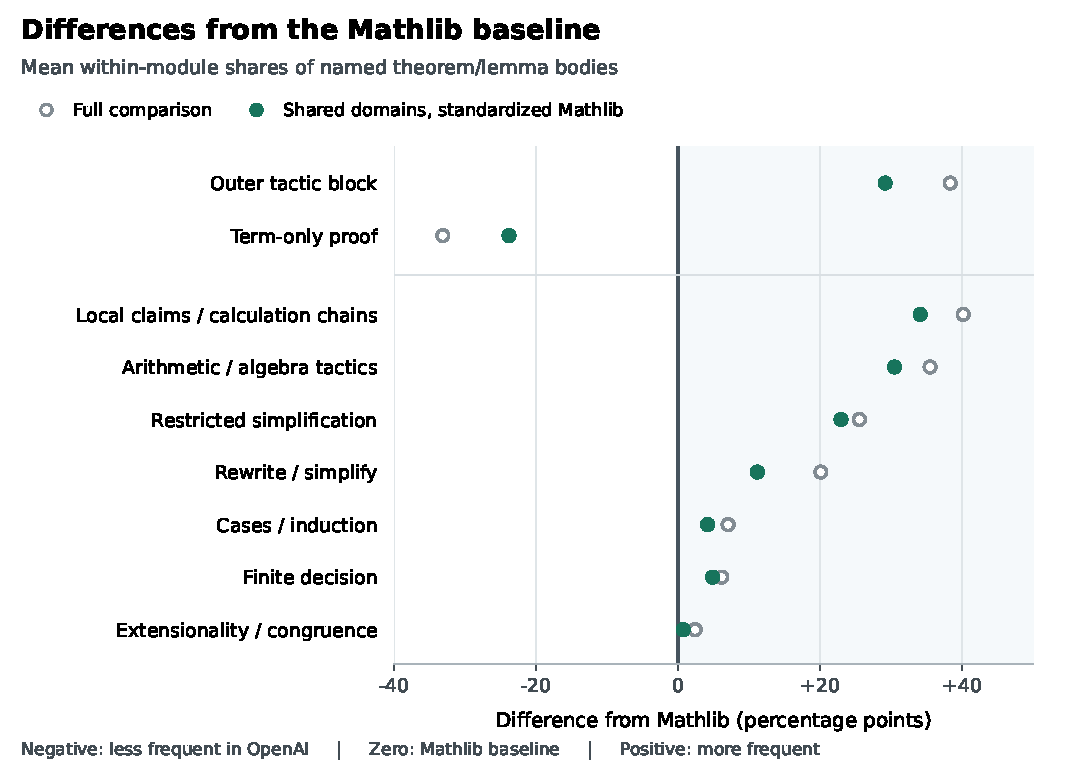
\includegraphics[width=\textwidth]{figures/method-shift.pdf}
\caption{OpenAI minus Mathlib differences in written proof-feature
prevalence, in percentage points. Zero denotes equal prevalence;
positive values indicate greater prevalence in the OpenAI sample.
Hollow markers compare all proof-bearing modules (784 OpenAI and
7,348 Mathlib). Green markers retain 735 OpenAI modules in 18 shared
domains and reweight Mathlib to the OpenAI domain shares. Both markers
lie at the same height for each feature and denote separate estimates
of the difference from Mathlib. Both comparisons average within-module
proof-body shares; features overlap except for the proof-mode
categories. The figure shows point estimates. Table~\ref{tab:profile}
reports absolute rates and 95\% OpenAI sampling intervals for selected
features in the full comparison. Table~\ref{tab:joint-profile} adds joint
subject and proof-length standardization.}
\label{fig:method-shift}
\end{figure}


Proof length changes the interpretation further. We jointly stratify by
the shared directory domains and four bands of nonempty body lines:
1--3, 4--10, 11--30, and 31 or more. The underlying measure remains
uniform selection of a proof-bearing module followed by a body within
it. Within a cell, a module's contribution is therefore proportional to
the fraction of its bodies in that cell. Mathlib's conditional feature
rates are reweighted to the OpenAI cell probabilities. This preserves
the module/body interpretation of Table~\ref{tab:profile}. The 69 shared
cells cover 93.75\% of that OpenAI measure.

For a feature $f$, write $\mu_C(f\mid s)$ for its conditional probability
in cell $s$ under corpus $C$, and let $w_s$ be the OpenAI cell probability
normalized over shared cells. The adjusted difference in percentage
points is
\[
  \Delta_f=100\sum_s w_s
  \bigl(\mu_{\mathrm{OpenAI}}(f\mid s)
       -\mu_{\mathrm{Mathlib}}(f\mid s)\bigr).
\]
Table~\ref{tab:joint-profile} compares this joint adjustment with the
subject-only results. Its exploratory intervals use 1,500 resamples of
OpenAI modules, recomputing their cell weights while keeping Mathlib's
cell means fixed.

\begin{table}[H]
\centering\small
\caption{OpenAI minus Mathlib differences in percentage points, with subject-only and joint subject/length standardization. Both use the module/body sampling measure. The 95\% percentile-bootstrap intervals resample OpenAI modules with Mathlib cell means fixed. The joint comparison covers 69 cells and 93.75\% of the OpenAI measure.}
\label{tab:joint-profile}
\setlength{\tabcolsep}{4pt}
\renewcommand{\arraystretch}{1.18}
\begin{tabular}{@{}p{6.0cm}rrr@{}}
\toprule
Written feature & Subject only & Subject + length & 95\% joint interval \\
\midrule
Outer tactic block & +29.2 & +10.4 & 9.3--11.5 \\[5pt]
Local claims or calculation chains & +34.1 & +5.8 & 4.4--7.3 \\[5pt]
Arithmetic or algebra tactics & +30.5 & +22.8 & 20.3--25.4 \\[5pt]
Restricted simplification & +22.9 & +7.7 & 5.4--9.8 \\[5pt]
Finite decision & +4.9 & +4.3 & 3.0--5.9 \\[5pt]
\bottomrule
\end{tabular}
\end{table}


Arithmetic and algebra tactics retain a difference of 22.8 percentage
points. The tactic-mode difference becomes 10.4 points and the
local-claim difference 5.8, compared with 29.2 and 34.1 under subject-only
adjustment. Thus proof-length composition is associated with much of
the latter contrasts. Length may itself reflect how an argument is
written, so conditioning on it changes the descriptive question.
The two comparisons show both the overall profile within subjects and
the remaining differences within broad subject/length cells.

Additional sensitivity checks remove each sampled directory-family group
in turn. The OpenAI arithmetic rate remains between 37.0\% and 38.7\%,
against 38.2\% in the full module-balanced sample. These groups are rough
proxies for developments; their exclusion shows that a single sampled
group does not account for the arithmetic profile. The retained data
also include the original pooled length-band comparison and alternative
family weights. Matching analogous mathematical tasks and declaration
roles would give a more specific baseline.

The listed general proof-search tokens, including \src{aesop},
\src{grind}, and \src{solve\_by\_elim}, have module-balanced rates of
0.07\% in the OpenAI sample and 3.35\% in Mathlib. Arithmetic tactics and simplification are themselves
automation, and other search tactics or imported macros can escape this
list. Similarly, \texttt{simp only} records explicit control of the rewrite
set. Its maintenance value depends on the surrounding proof. Mathlib's
guidance treats squeezing terminal simplification calls as a tradeoff
involving performance and fragility \citep{MathlibStyle}.

\subsection{Why certificate batches change the apparent distribution}

Concentration makes the distinction between modules and bodies essential.
Ten sampled OpenAI modules contribute 48.2\% of the extracted bodies;
the largest alone contributes 14.9\%. Consequently the pooled
finite-decision rate is 48.9\%, compared with the module-balanced 6.3\%.
Pooled rewrite/simplification rates are 41.5\% versus Mathlib's 48.8\%,
even though the module-balanced ordering in Table~\ref{tab:profile} is
reversed. Pooled rates describe the produced body population; module
averages describe practice under the module/body selection measure.

Reading these large files reveals an informative construction. The
sampled planar-packing module \src{LowBlock36\_10} contains 872 named
bodies, 792 of which contain a finite decision.\footnote{Source:
\href{https://github.com/openai/math/blob/fd4aeeb2ee4fc729c18d98444fed42fd0529eeeb/lean/OAI/Analysis/PlanarPacking/Certificate/LowBlock36_10.lean\#L16-L67}{\src{Analysis/PlanarPacking/Certificate/LowBlock36\_10.lean}, lines 16--67}.}
It defines exact integer interval data, checks individual entries with
\texttt{decide +kernel}, and assembles them into finite sums. A sampled
transonic barrier module chains Horner-step certificates with previously
proved tail bounds.\footnote{Source:
\href{https://github.com/openai/math/blob/fd4aeeb2ee4fc729c18d98444fed42fd0529eeeb/lean/OAI/MathematicalPhysics/Transonic/Certificates/Barrier59.lean\#L675-L678}{\src{MathematicalPhysics/Transonic/Certificates/Barrier59.lean}, lines 675--678}.}
The construction places exact data and small checks beneath soundness
and assembly lemmas. Lean 4.34.1 documents \texttt{decide +kernel} as
evaluating the decision instance by kernel reduction
\citep{LeanDecideSource}. This mechanism explains how a large collection
of short proofs serves as a numerical certificate for a later estimate.

The persistent arithmetic difference and the separate certificate layer
provide the clearest empirical findings. The larger unadjusted contrasts
also describe differences in proof form and length composition. Read
alongside the cases, these results motivate a division-of-work account:
preservation interfaces prepare mathematical obligations, and established
Lean devices check the resulting local steps. Section~\ref{sec:tactics-synthesis}
traces this interaction in particular proof bodies.

\section{Worked examples: why the stronger interface matters}
\label{sec:worked}

The first three examples unpack the common-base case: selecting random
bits, preserving the output law, and composing an error budget. The
remaining examples return to boundary locality, trace limits, and named
coordinates. Each isolates the information needed by a later operation
without the surrounding formal development.

\subsection{Injective tape positions preserve a uniform experiment}
\label{sec:tape-example}

\begin{samepage}
\begin{proposition}\label{prop:tape}
Let $p:\{0,\ldots,m-1\}\to\{0,\ldots,B-1\}$ be injective. If
$\beta$ is uniform on $\{0,1\}^B$, then
$(\beta(p(0)),\ldots,\beta(p(m-1)))$ is uniform on $\{0,1\}^m$.
Every word has exactly $2^{B-m}$ preimages.
\end{proposition}
\begin{proof}
Prescribing the $m$ selected bits leaves precisely $B-m$ coordinates
free. Each assignment to these remaining coordinates determines one
preimage. Thus every word has the same number of preimages, and its
probability is $2^{B-m}/2^B=2^{-m}$.
\end{proof}
\end{samepage}

For the common-base machine, the relevant map is
$p(i)=s+3(m-1-i)+1$. Reversal and multiplication by three preserve
distinctness. For $i<m$, its value is less than $B$ whenever
$s+3m+1\leq B$. The latter bound is stronger than needed for the selected
positions because it also accounts for the surrounding execution.
The review's Lean file proves these arithmetic facts for arbitrary natural
$s,m,B$, including the empty-word case.

\Needspace{7\baselineskip}
The index map is defined by
\begin{lstlisting}
def physicalIndex (start m : Nat) (i : Fin m) : Nat :=
  start + 3 * (m - 1 - i.val) + 1
\end{lstlisting}
The proof uses the bounds stored in \src{Fin m} to justify subtraction
arithmetic. This matters: natural-number subtraction is truncated, so
injectivity would fail on unrestricted natural indices. A range type is
part of the mathematical interface, not a cosmetic annotation.

For comparison, if $p(0)=p(1)$, the words $01$ and $10$ have no
preimages. Reading fair individual bits does not by itself produce an
independent word. Proposition~\ref{prop:tape} explains why the source proves
injectivity of the physical positions before transporting the success
probability. The Python companion exhaustively checks 15 small choices
of $(s,m,B)$ against the exact fiber count.

\subsection{Observables determine a finite law; its mean does not}
\label{sec:law-example}

\begin{samepage}
\begin{proposition}\label{prop:law}
Let $\mu,\nu$ be probability measures on a finite set $X$. Then
$\E_\mu\varphi=\E_\nu\varphi$ for every $\varphi:X\to\R$ if and only
if $\mu=\nu$.
\end{proposition}
\begin{proof}
For each $x\in X$, take $\varphi=\mathbf1_{\{x\}}$ to obtain
$\mu(\{x\})=\nu(\{x\})$. Summing singleton masses gives equality on every
subset. The converse follows from the definition of finite expectation.
\end{proof}
\end{samepage}

In a uniform finite experiment, these expectations are normalized sums
with integer multiplicities. The Lean companion proves the corresponding
count statement: equality of unnormalized sums against every natural-valued
observable determines each multiplicity. If two sampling spaces have
different cardinalities $N,N'>0$, equality of their output laws instead
means $N'c(x)=Nc'(x)$ for each output $x$. The companion also proves this
cross-multiplied statement from equality of normalized observables.
For example, multiplicities $(1,1,1)$ and $(2,2,2)$ describe the same law,
although their unnormalized counts differ. It then checks the measures on
$X=\{0,1,2\}$ with multiplicities
\[
  (1,1,1)\quad\text{and}\quad(0,3,0).
\]
Both have total mass three and mean one after normalization. Their
probabilities of $\{0\}$ are $1/3$ and zero. Thus preservation of the
expected numerical output would be insufficient for an accuracy event.
The universal observable certificate in Section~\ref{sec:common-bases}
supports exactly the stronger conclusion required: substitute the
indicator of the desired relative-error interval.

This interpretation also explains why the source allows reindexing of
draw outcomes. A permutation can change the result returned for a
particular numbered bank without changing its distribution under uniform
sampling. Law equality is the appropriate interface between those
experiments; the deterministic compiler layer separately preserves the
execution result for a supplied bank.

\subsection{From a bounded experiment to a finite success count}
\label{sec:success-budget}

The preceding two interfaces can be composed with a quantitative error
bound. This gives a concrete way to read the final accuracy statement of
Section~\ref{sec:common-bases}.

\begin{samepage}
\begin{proposition}\label{prop:success-budget}
Let $X$ be finite, adjoin a failure symbol $\bot$, and let $U$ be an
ideal $X$-valued output. Let $V$ be a bounded implementation driven by a
uniform $m$-bit word, taking values in $X\cup\{\bot\}$.
For $\varphi:X\to[0,1]$, set
$\varphi(\bot)=0$. Suppose
\[
  \E\varphi(V)\geq\E\varphi(U)-\eta
  \quad\text{for every such }\varphi.
\]
Let $\eta,\delta_0\geq0$ and
$A\subseteq X$ satisfy $\Pr(U\in A)\geq1-\delta_0$.
If a machine obtains its word from fixed injective positions in a
uniform $B$-bit tape and returns $V$ on that word, then
\[
  \#\{\text{successful }B\text{-bit tapes}\}
  \geq(1-\delta_0-\eta)2^B,
\]
where success means returning an element of $A$.
\end{proposition}
\begin{proof}
Choose $\varphi=\mathbf1_A$ to obtain
$\Pr(V\in A)\geq1-\delta_0-\eta$. Proposition~\ref{prop:tape}
shows that the tape projection has the required uniform word law.
Multiplying its success probability by $2^B$ gives the count.
\end{proof}
\end{samepage}

For a single accuracy event, only its indicator is needed; the
all-observables hypothesis makes the estimate reusable for other events.
In the source's bounded draw-tree implementation, the fit condition
requires at most $M$ successive draws and $H\geq\lceil\log_2 a\rceil$
trial bits for every draw arity $a$. With $D$ trials per draw,
$\eta=M2^{-D}$, with failed runs assigned
observable value zero.\footnote{See
\href{https://github.com/openai/math/blob/fd4aeeb2ee4fc729c18d98444fed42fd0529eeeb/lean/OAI/Combinatorics/MatroidCounting/CommonBases.lean\#L9346-L9349}{\src{CommonBases.lean}, \src{run_lower}}.}
For a desired failure budget $0<\delta<1$, choosing
$\delta_0\leq\delta/2$ and $M2^{-D}\leq\delta/2$ suffices.
When $M>0$, one may take
$D\geq\max\{0,\lceil\log_2(2M/\delta)\rceil\}$.
The required tape length and execution bound must still be proved
separately. Thus the accuracy budget, the uniformity of the gathered
bits, and the deterministic machine specification are distinct inputs
to a single final guarantee.

A tight finite example joins the layers. Let the ideal probabilities of
$a,b$ be $6/8,2/8$, and assign the eight implementation words to five
copies of $a$, two of $b$, and one failure. The observable loss is exactly
$\varphi(a)/8$, hence at most $\eta=1/8$. For $A=\{a\}$,
$\delta_0=1/4$ and the lower bound is $5/8$. Embedding the three-bit word
at positions $7,4,1$ in a ten-bit tape gives exactly
$5\cdot2^7=640$ successful tapes out of $1024$. The Python companion
enumerates those tapes and all event indicators. This fixture illustrates
the composed bound independently of the upstream rejection sampler.

\subsection{Boundary values and ambient derivatives}
\label{sec:local-forms}

The Mahler case uses local equality to identify ambient derivatives.
On $\R^2$, the
one-forms $\omega=0$ and $\eta=(x^2+y^2-1)\,dx$ agree at every point
of the unit circle. Their ambient exterior derivatives need not agree:
$d\eta=-2y\,dx\wedge dy$, which is nonzero at $(0,1)$.
Equality on a neighborhood does imply equality of the ambient derivatives.
The Mahler cutoff argument uses this sufficient condition to transfer
its ambient derivative; agreement on tangent arguments suffices for the
later comparison of integration densities. Intrinsic differentiation
after pullback to the circle uses different data: both pulled-back forms,
and their exterior derivatives, vanish. Mathlib's
differential-form interface explicitly uses the derivative of a
form-valued field \citep{MathlibForms}.


\subsection{A cut-sensitive limit that is not pointwise}
\label{sec:trace-example}

Consider the commutative $C^*$-algebra $c_0$ of complex sequences tending
to zero, with pointwise operations and the supremum norm. On its positive
cone define
\[
  \tau(a)=\sum_{j=1}^{\infty}a_j\in[0,\infty].
\]
The trace is additive, positively homogeneous, and tracial. It is lower
semicontinuous because it is the supremum of its continuous finite partial
sums. Finite-support sequences belong to $\mathcal N_\tau$, so the closed
finite ideal $I_\tau$ in~\eqref{eq:finite-ideal} is all of $c_0$.

For every positive $a\in c_0$ and $\varepsilon>0$, the sequence
$(a-\varepsilon)_+$ has finite support. Consequently
\[
  \lim_{r\downarrow0}r\tau((a-\varepsilon)_+)=0,
  \qquad 0\leq\liminf_{r\downarrow0}r\tau(a).
\]
These are precisely the two inequalities in
\eqref{eq:trace-canonical-convergence} with limit trace
$\iota_{c_0}=0$. But for $a_j=1/j$ one has $\tau(a)=\infty$, hence
$r\tau(a)=\infty$ for every $r>0$. The pointwise limit at this element
is infinity. The finite ideal and canonical limit are nevertheless
unambiguous.

This classical example makes the reason for the positive cuts concrete
\citep{ElliottRobertSantiago2011}. Closure admits elements with infinite
trace, while every fixed positive cut is controlled by a finite value.
Replacing the source's convergence predicate by pointwise convergence
would therefore alter the theorem.


\subsection{Equal flags and different named coordinates}
\label{sec:named-maps}

The character-variety case preserves more than the flag of subspaces.
Two frames of a one-dimensional vector space can induce the
same flag but different named coordinate maps. If $e(u)=uv$ and
$f(u)=2uv$ over a field of characteristic zero, both give the flag
$0\subset\operatorname{span}(v)$, while
$e^{-1}(v)=1$ and $f^{-1}(v)=1/2$. The all-seams predicate must therefore
retain the named graded maps when those maps occur in the seam equation.
The coordinate equation consumes information that equality of the
underlying flag has forgotten. This is the small-scale reason for
retaining named graded maps throughout the surface construction.

\section{Discussion: interfaces and the division of proof work}
\label{sec:discussion}

\subsection{What the mathematical comparison reveals}

The downstream operation determines what a preservation statement must
expose. Transferring an accuracy guarantee requires the relevant event
probability; equality of output laws supports all such transfers.
A named-coordinate equation uses the coordinate map. Ambient
differentiation uses local information about a field. A sharp norm
estimate uses the normalization and weights of the preceding bounds.
Exact data, laws, estimates, and local differential information can
therefore appear together in one development.

The most informative transitions occur when the next operation changes
these requirements. The common-base proof preserves a distribution
through reindexing, then execution on each supplied bank. Mahler
identifies form-valued fields for differentiation, then uses tangential
agreement for boundary integration. Trace-cone reconstruction obtains
ideal order from addition, then uses convergence and scaling to identify
the ideals of a particular trace. Following the next operation explains
why each interface has its particular fields.

Implementation details sharpen the comparison. Encoded width and
numerical attributes answer different complexity questions in the
compiler. The graph restriction identity restores the counting norm
when local assignment estimates are summed. Image filters extend a
carrier-indexed convergence property to arbitrary nets. These choices
expose mathematical data through lemmas that later constructions can
reuse. The compiled ideal-composition example in
Section~\ref{sec:upstream-reuse} demonstrates this reuse directly.

Two cases show how a local calculation controls a global estimate.
The graph's total-two table isolates an exceptional direction whose
aggregate energy is paid for by switch gains. In Crouzeix, rectangular
compressions and two orders of polynomial multiplication produce
compatible energy bounds. The final scalar cancellation is short because
the earlier constructions have supplied its exact constants and signs.

These patterns have substantial antecedents. Verified compilers establish
semantic preservation between source and implementation
\citep{Leroy2009,CakeML2014}; probabilistic program logics reason about
distributions and observations \citep{CertiCrypt2009,EasyCrypt2011}.
Algebraic hierarchy design and specification-driven collaboration make
interfaces part of mathematical construction
\citep{GarillotEtAl2009,Baanen2022,CommelinTopaz2024}. The present
comparison identifies what those interfaces preserve in the selected
proofs and how their composition supplies a later calculation's inputs.

\subsection{Tactic use and the division of proof work}
\label{sec:tactics-synthesis}

The corpus survey adds a measured comparison of written proof practice.
After joint subject and proof-length standardization, arithmetic and
algebra tactics remain more prevalent by 22.8 percentage points. Tactic
mode and local claims retain differences of 10.4 and 5.8 points,
respectively. The larger subject-only contrasts in
Figure~\ref{fig:method-shift} also reflect proof-length composition;
Table~\ref{tab:joint-profile} makes that distinction explicit. Arithmetic
emphasis is the clearest persistent difference among these features.

The common-base fold-cost proof shows how such local automation fits
into a semantic argument. Execution identities justify applying the
induction hypothesis to the remaining fold. The safety invariant and
width bound supply its premises. The following consecutive source lines
then apply that hypothesis and close the cost inequality:\footnote{Source:
\href{https://github.com/openai/math/blob/fd4aeeb2ee4fc729c18d98444fed42fd0529eeeb/lean/OAI/Combinatorics/MatroidCounting/CommonBases.lean\#L16880-L16907}{\src{CommonBases.lean}, lines 16880--16907}; excerpt, lines 16905--16907.}
\begin{lstlisting}[caption={Lean source excerpt: fold induction followed by arithmetic discharge.},label={lst:fold-cost}]
have hh := ih z' y' e (hs.2 z' hrun) hw' ht
simp only [List.length_cons,Nat.add_mul,Nat.one_mul]
omega
\end{lstlisting}
Here \src{hs.2} supplies safety after the accumulator update, and
\src{hw'} bounds the remaining list's width. Expanding the successor
length exposes shared product terms. Although the displayed cost bound
contains multiplication, the remaining comparison fits linear
natural-number arithmetic. The semantic and size arguments prepare the
obligation that \src{omega} checks.

\Needspace{14\baselineskip}
The Crouzeix proof supplies a parallel example in analysis. Fourier and
positive-block estimates have already produced bounds with the same
energy $a$ and norm $\gamma$. Their closing scalar argument is:\footnote{Source:
\href{https://github.com/openai/math/blob/fd4aeeb2ee4fc729c18d98444fed42fd0529eeeb/lean/OAI/Analysis/DirectCrouzeix/DomainCore.lean\#L105-L117}{\src{DirectCrouzeix/DomainCore.lean}, lines 105--117}; excerpt, lines 111--117.}
\begin{lstlisting}[caption={Lean source excerpt: the closing Crouzeix energy calculation.},label={lst:crouzeix-close}]
have hb : 2*a ≤ 8*a/γ^2 := by
  simp only [mul_div_assoc] at hPE hQE ⊢
  linarith
have hmul := (le_div_iff₀ (sq_pos_of_pos hγ)).mp hb
change γ ≤ 2
have hg2 : γ^2 ≤ 4 := by nlinarith [hapos]
nlinarith
\end{lstlisting}
The first tactic combines the available energy inequalities. Positivity
of $\gamma$ then permits denominator clearing, and positivity of $a$
permits the final cancellation. The choice of compressions, Fourier
weights, and zero-mode identities creates the relations that these
arithmetic steps certify.

Exact numerical certificates exhibit a further division of work. Their
finite checks verify retained interval data; assembly and soundness
lemmas explain why those checks imply the required estimate. Across
these examples, representation design and local automation meet at an
explicit obligation with proved hypotheses. The survey establishes a
broader method profile, while the case tracing explains mechanisms
within completed source proofs. Testing effects on completion rates,
development effort, or maintenance would require matched tasks and
corresponding outcome measurements.

\subsection{Proof generation, simplification, and mathematical explanation}
\label{sec:generation-explanation}

The comparison identifies differences between completed source corpora.
Mathlib is a collaborative library with varied authoring histories, rather
than a controlled sample of unaided human proofs. These data therefore
cannot establish a distinct AI reasoning process, an advantage in
completion time, or a superior method of doing mathematics. They suggest
a workflow hypothesis: automation may be especially effective when
proved interfaces expose many local obligations in forms handled by
existing tactics. The relevant conditions---available representations,
library coverage, and checkable local goals---can vary within a subject
as well as between subjects. Interface construction remains part of the
work whose cost must be measured.

Obtaining a checked proof and obtaining an economical explanation are
separate objectives. ProofOptimizer reports substantial token
reductions in generated Lean proofs, using Lean to check replacements
against the original theorem statements \citep{GuEtAl2025ProofOptimizer}. Lean Refactor studies proof
length, compilation cost, and compatibility across library versions as
distinct optimization objectives \citep{LuEtAl2026LeanRefactor}. These
results indicate scope for refactoring on the evaluated benchmarks;
they do not measure redundancy in the six
developments examined here. Shorter tactic scripts can also invoke
heavier automation. Source length, proof-checking cost, dependency
structure, and explanatory clarity should consequently be assessed
separately.

Together these observations motivate a research direction: connect
proof generation to compression, reusable interfaces, and mathematical
explanation. A useful interface may amortize its construction cost over
many later results, while a concise final proof may conceal substantial
setup. Claims of improved mathematical practice require evidence about
total effort, generality, downstream reuse, and reader understanding,
alongside correctness. The present findings locate possible mechanisms
and evaluation targets without establishing those improvements.

\subsection{Using the comparison in a new formalization}

Begin with the quantity the next theorem consumes: an event probability,
a coordinate equation, a derivative, or an inequality. Identify what a
proposed representation changes, such as multiplicities, coordinate
order, multiplication order, or the neighborhood of definition. The
preservation statement should connect those changed data to that
specific quantity.

The worked examples make the choice concrete. An event indicator is
sufficient to transfer one accuracy probability, while a full output-law
identity supports reuse for other events. Neighborhood agreement
identifies ambient derivatives; tangential agreement can suffice for the
later integral. A named seam equation needs its coordinate maps.
Proposition~\ref{prop:success-budget} combines several interfaces in one
count: implementation loss, tape uniformity, and deterministic execution
jointly yield the success guarantee.

Next, follow how the hypotheses are supplied for the actual inputs.
Mahler's strip maps construct the analytic data, and Crouzeix's outer
domains provide strict containment and the required estimates. In the
marked-surface construction, one splitting witness supplies both the
diagram and its coordinate identifications. The reusable design consists
of a precise local model, a preservation relation, and a construction of
the data required to apply it.

Finally, inspect the local goals exposed by that design. A width
invariant can reduce a compiler cost step to natural-number arithmetic.
Positive denominators and nonzero factors can prepare an analytic
cancellation. Exact interval data can make a numerical obligation
decidable. The interface proofs assign established automation a concrete
part of the larger mathematical argument to check.

\subsection{Scope and further work}

The six cases were selected for interfaces that could be traced in depth.
Their mathematical comparisons are complemented by the separate uniform
module sample. Joint domain/length controls and directory-family
sensitivity checks sharpen the survey's descriptive interpretation.
A comparison of analogous declaration roles and mathematical tasks would
further separate library composition from choices about proof organization.
Elaborated tactic traces and a held-out extraction-validation cohort
would connect the lexical measurements more directly to executed proof steps.
A prospective comparison could cross AI assistance with availability of
proved representation interfaces on matched tasks, retaining unsuccessful
attempts. Relevant outcomes include time to a checked proof, human
intervention, inference and checking costs, later reuse, and blinded
expert assessments of clarity. This would test the workflow hypothesis
without treating completed-proof length as a causal control.

Source reading identifies the inspected declarations, their hypotheses,
and the constructions connecting them. Compilation of the worked
examples and the three-module trace-cone reuse experiment supplies
additional checking evidence at those targets. Rebuilding the remaining
case endpoints and examining their mathematical arguments would extend
this assessment. Endpoint statements and support results retain their
distinct roles throughout the comparison.

For readers of substantial Lean developments, the practical route is to
locate the next operation, identify what it consumes, and follow the
theorem preserving that information. For formalizers, the cases show how
interface design prepares local proof obligations. The corpus comparison
adds evidence about which written devices are prevalent in this
collection, with arithmetic emphasis persisting under coarse joint
controls. The review brings these two levels together: the mathematical
content of preservation statements and the local proof work they support.

\Needspace{24\baselineskip}
\section*{Data and code availability}

The accompanying reproduction repository (release~1.6.0) provides the
manuscript source, data, and analysis code \citep{GounderArchitectureData2026}.
The source package contains the LaTeX manuscript, reference records,
declaration ledgers, original Lean examples, and Python checks. Five
elementary Lean lemmas import only \src{Lean}. The upstream reuse
experiment imports \src{OAI.Analysis.TraceCone.IdealTransport} and compiles
its three-module dependency chain from unchanged source bytes. Both use
Lean 4.34.1; the latter uses Mathlib revision
\src{d13f23b723b8a846827a245b89c10fc7d3f11612}. Compiler logs retain the
reported axioms. Exact Python checks enumerate tape fibers and Boolean
matrix counts. The README gives reproduction commands and identifies the
external dependencies.

The method-survey directory retains the complete path population, all
800 sampled source modules and their hashes, extraction tables, feature
definitions, bootstrap summaries, and forty inspected validation cases.
The joint comparison additionally retains cell weights, conditional
rates, intervals, and the generated manuscript table. Baseline profiling
requires the pinned Mathlib source checkout; the lexical survey reads
source without elaborating the developments. Public manuscript source
links resolve to the reviewed repository revision.

The source inventory is the complete Git tree of \src{openai/math},
inspected on 8 October 2026.\footnote{Reviewed revision:
\src{fd4aeeb2ee4fc729c18d98444fed42fd0529eeeb}. Public source links refer
to that revision.} It contains 122,875 files with the \src{.lean}
extension, including supporting modules. The package retains 546 source
artifacts, including the \src{OAI} import closures for the six selected
cases; twenty-one detailed records document the additional proof-body
analysis. The separate formalization catalogue lists 173 source records
and 200 main-result bindings \citep{OAICatalog}. These inventories count
different objects and should be read alongside their stated units.

The collection also supplies Comparator challenge configurations
\citep{OAIComparator}. The inspected checker implements statement
comparison, dependency and axiom inspection, kernel replay, and an
optional external checker \citep{ComparatorSource2026}.\footnote{Checker
source revision: \src{ca04cfc72b550331658ec314bf47685281bfd4bf}. This
records the infrastructure source inspected; the collection's
installation instructions do not specify that revision.}
The distinction between proof construction and checking has a long
history \citep{deBruijn1970,BarendregtWiedijk2005}; Lean typechecker
verification supplies a contemporary example \citep{Carneiro2025Lean4Lean}.
Library maintenance addresses consistency across a growing development
\citep{vanDoornEbnerLewis2020}. Interpreting the mathematics additionally
requires reading the formal objects and hypotheses, the task pursued
by the case studies here.

\section*{Generative AI disclosure}
OpenAI Codex agents contributed substantially to source discovery, literature synthesis, and mathematical exposition.
\begingroup
\setlength{\bibsep}{4pt}
\bibliographystyle{plainnat}
\bibliography{references}
\endgroup
\end{document}
